\section{Closest pair of points}
\label{sec:closest_pair_of_points}


\begin{frame}
	\frametitle{A new problem}
	\begin{problemblock}{Closest pair of points}
		Given a set of points, what is the pair of points that is closest to each other?\\
		\pause
		More formally:
		\begin{itemize}
			\item Given a set of points $S$, where every point $p_i$ has an x-coordinate $x_i$ and y-coordinate $y_i$.
			\item Distance is defined as: $d(i,j) = \sqrt{{(x_i - x_j)}^{2} + {(y_i-y_j)}^2}$
			\item What is the pair of points $i,j$ such that $d(i,j)$ is minimal?
		\end{itemize}
	\end{problemblock}
	\pause
	\section{Closest pair of points}
\label{sec:closest_pair_of_points}


\begin{frame}
	\frametitle{A new problem}
	\begin{problemblock}{Closest pair of points}
		Given a set of points, what is the pair of points that is closest to each other?\\
		\pause
		More formally:
		\begin{itemize}
			\item Given a set of points $S$, where every point $p_i$ has an x-coordinate $x_i$ and y-coordinate $y_i$.
			\item Distance is defined as: $d(i,j) = \sqrt{{(x_i - x_j)}^{2} + {(y_i-y_j)}^2}$
			\item What is the pair of points $i,j$ such that $d(i,j)$ is minimal?
		\end{itemize}
	\end{problemblock}
	\pause
	\section{Closest pair of points}
\label{sec:closest_pair_of_points}


\begin{frame}
	\frametitle{A new problem}
	\begin{problemblock}{Closest pair of points}
		Given a set of points, what is the pair of points that is closest to each other?\\
		\pause
		More formally:
		\begin{itemize}
			\item Given a set of points $S$, where every point $p_i$ has an x-coordinate $x_i$ and y-coordinate $y_i$.
			\item Distance is defined as: $d(i,j) = \sqrt{{(x_i - x_j)}^{2} + {(y_i-y_j)}^2}$
			\item What is the pair of points $i,j$ such that $d(i,j)$ is minimal?
		\end{itemize}
	\end{problemblock}
	\pause
	\section{Closest pair of points}
\label{sec:closest_pair_of_points}


\begin{frame}
	\frametitle{A new problem}
	\begin{problemblock}{Closest pair of points}
		Given a set of points, what is the pair of points that is closest to each other?\\
		\pause
		More formally:
		\begin{itemize}
			\item Given a set of points $S$, where every point $p_i$ has an x-coordinate $x_i$ and y-coordinate $y_i$.
			\item Distance is defined as: $d(i,j) = \sqrt{{(x_i - x_j)}^{2} + {(y_i-y_j)}^2}$
			\item What is the pair of points $i,j$ such that $d(i,j)$ is minimal?
		\end{itemize}
	\end{problemblock}
	\pause
	\input{figures/tikz/closestpair.tex}
	\pnote{Why is this relevant? Answers: For instance collision detection algorithms}
\end{frame}

\begin{frame}
	\frametitle{Let's just brute-force it?}
	\begin{overlayarea}{\textwidth}{\textheight}
		\input{figures/tikz/closestpair.tex}
		\begin{questionblock}{Brute-force}
			What is the tightest upper bound on the run time for a brute-force solution given $|S| = n$?
			\only<2>{
			\begin{enumerate}[A.]
				\item $O(n \log n)$
				\item $O(n^2)$
				\item $O(n^2 \log n)$
				\item $O(n^3)$
				\item I don't know.
			\end{enumerate}
		}
		\end{questionblock}
		\only<3>{
			\begin{answerblock}{Try every combination}
				We check every pair of points, of which there are $n^2$, so $O(n^2)$.	
			\end{answerblock}
		}
	\end{overlayarea}
\end{frame}

\begin{frame}
	\frametitle{Time to improve!}
	\framesubtitle{Using Divide \& Conquer}
		\begin{columns}
			\column{0.455\textwidth}
			\begin{center}
				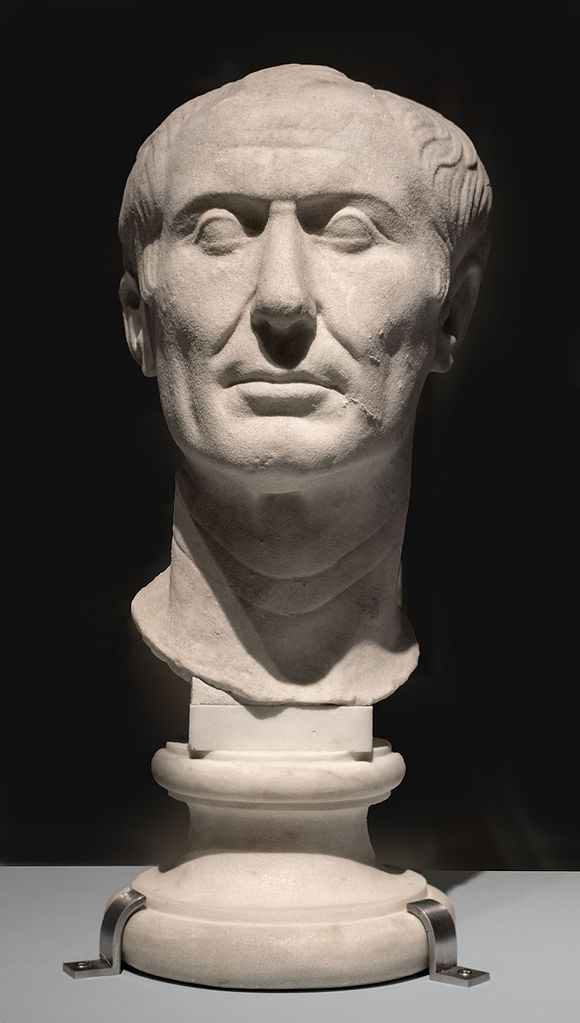
\includegraphics[width=0.5\textwidth]{figures/ceasar.jpg}\\
				\hspace*{15pt}\hbox{\scriptsize Image By:\thinspace{\itshape Ángel M. Felicísimo}}
				%https://commons.wikimedia.org/wiki/File:Retrato_de_Julio_C%C3%A9sar_(26724093101).jpg
			\end{center}

			\column{0.455\textwidth}
			\begin{center}
				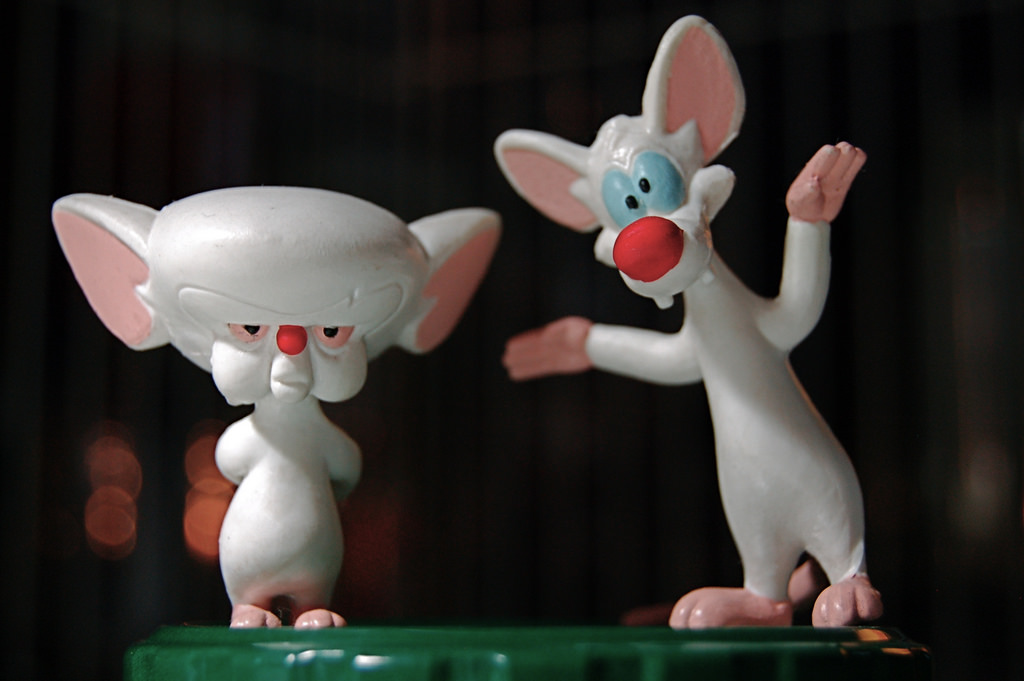
\includegraphics[width=0.9\textwidth]{figures/pinky.jpg}\\
				\hspace*{15pt}\hbox{\scriptsize Image By:\thinspace{\itshape JD Hancock}}
				%https://commons.wikimedia.org/wiki/File:Retrato_de_Julio_C%C3%A9sar_(26724093101).jpg

			\end{center}
		\end{columns}
\end{frame}

\begin{frame}
	\frametitle{Ideas for an algorithm}

	\begin{overlayarea}{\textwidth}{\textheight}
		\input{figures/tikz/closestpair_fixed.tex}
		
		\pause
		\begin{exampleblock}{Algorithm}
			\begin{itemize}
				\item \alert<2>{Divide}: Draw vertical line $L$ that has roughly half of the points on each side.
					\pause
				\item \alert<3>{Conquer}: Find the closest pair on each side.
					\pause
				\item \alert<4>{Combine}: Find the closest pair with one point on each side.
					\pause
				\item Return the minimum of these 3.
			\end{itemize}
		\end{exampleblock}	
	\end{overlayarea}
\end{frame}

\begin{frame}
	\frametitle{Did we make things better?}
	\begin{questionblock}{What is the run time of combine?}
		How much time to combine the two halves? Remember that we want to improve over $\Theta(n^2)$.
	\end{questionblock}	
\end{frame}

\begin{frame}
	\frametitle{How do we make it better?}
		\input{figures/tikz/closestpair_fixed2.tex}
	Observation:
	\begin{itemize}
		\item If $\delta$ is the minimum of the smallest distances left and right.
			\pause
		\item Then we only need to consider pairs of points within $\delta$ of $L$.
			\pause
		\item So in this example, none at all!
	\end{itemize}
\end{frame}

\begin{frame}
	\frametitle{Worst-case?}
	\begin{overlayarea}{\textwidth}{\textheight}
			\begin{itemize}
				\item But worst-case all points are in this $2\delta$-strip...
					\pause
				\item But if we sort them by $y$-coordinate (which can be done in $O(n\log n)$), then how many comparisons do we need?
					\pause
				\item Still $O(n^2)$!?
					\only<4->{
				\item Nope! We only need to check within 11 (i.e. a constant number of) positions in the sorted list.
				}
					\only<5->{
				\item So the combining step is $O(n \log n)$ (which can be further improved to $O(n)$)!
				}
			\end{itemize}
			\only<3>{
			\begin{center}
				
\includegraphics[width=0.4\textwidth]{figures/dilbert.jpg}
				\framesubtitle{http://thecontextofthings.com/wp-content/uploads/2017/11/dilbert-work.jpg}
			\end{center}
		}
	\end{overlayarea}
\end{frame}

\begin{frame}
	\frametitle{Why 11?}

	\begin{overlayarea}{\textwidth}{\textheight}
		\begin{columns}
			\column{0.655\textwidth}
			\begin{block}{Definition}
				Let $s_i$ be the point in the $2\delta$-strip with the $i^\text{th}$ smallest $y$-coordinate.
			\end{block}	
			
			\pause
			\begin{block}{Claim about 11}
				If $|i-j| > 11$ then the distance between $s_i$ and $s_j$ is at least $\delta$.
			\end{block}
			\column{0.255\textwidth}
			\input{figures/tikz/closestpair_delta.tex}	
		\end{columns}
		
		\pause
		\only<3-5>{
			\begin{block}{Proof sketch}
			\begin{itemize}
				\item No two points are in the same $0.5\delta$-by-$0.5\delta$-box.
					\only<4->{
				\item Two points that have two rows between them have a distance $\geq 2\cdot(0.5\delta) = \delta$.
				}
				\only<5->{
				\item So we only consider points at most 2 rows away.
				}
			\end{itemize}
		\end{block}
	}
	\only<6->{
		\begin{exampleblock}{Fun facts!}
			\begin{itemize}
				\item We can even reduce this to just 7 points.
					\only<7>{
				\item Even less if we consider columns separately.
				}
			\end{itemize}
		\end{exampleblock}	
	}
		
		\only<3>{
		\begin{questionblock}{Why not?}
			Why are there no two points in the same box?
		\end{questionblock}
}
	\end{overlayarea}
\end{frame}

\begin{frame}
	\frametitle{The algorithm}
	\begin{columns}
		\column{0.705\textwidth}
	\begin{algorithmic}
		\State Sort all points by x-coordinate
		\Function{Closest-Pair}{$p_1,\dots,p_n$}
			\If{n=1}
				\State \Return $\infty$
			\EndIf

			\pause
			\State $L \gets$ \alert<2>{median} $x$-coordinate
			\State $\delta_1 \gets$ \Call{Closest-Pair}{Points left of $L$}
			\State $\delta_2 \gets$ \Call{Closest-Pair}{Points right of $L$}
			\State $\delta \gets \min(\delta_1,\delta_2)$
			\pause
			\State get list of all points within $\delta$ from L.
			\State sort this list by y-coordinate
			\pause
			\State Scan by y-order, compare every point to the next 11 and update $\delta$ as you go.
			\State \Return $\delta$
		\EndFunction
	\end{algorithmic}
		\pnote{Why not the average?}
		\column{0.205\textwidth}
		\pause
		\begin{questionblock}{}
			What is the recurrence equation for the run time?	
		\end{questionblock}	
		\pause
		\begin{answerblock}{}
			\small
			$T(n) =2T(n/2) + O(n\log n)$	
		\end{answerblock}
	\end{columns}
	
\end{frame}

	\pnote{Why is this relevant? Answers: For instance collision detection algorithms}
\end{frame}

\begin{frame}
	\frametitle{Let's just brute-force it?}
	\begin{overlayarea}{\textwidth}{\textheight}
		\section{Closest pair of points}
\label{sec:closest_pair_of_points}


\begin{frame}
	\frametitle{A new problem}
	\begin{problemblock}{Closest pair of points}
		Given a set of points, what is the pair of points that is closest to each other?\\
		\pause
		More formally:
		\begin{itemize}
			\item Given a set of points $S$, where every point $p_i$ has an x-coordinate $x_i$ and y-coordinate $y_i$.
			\item Distance is defined as: $d(i,j) = \sqrt{{(x_i - x_j)}^{2} + {(y_i-y_j)}^2}$
			\item What is the pair of points $i,j$ such that $d(i,j)$ is minimal?
		\end{itemize}
	\end{problemblock}
	\pause
	\input{figures/tikz/closestpair.tex}
	\pnote{Why is this relevant? Answers: For instance collision detection algorithms}
\end{frame}

\begin{frame}
	\frametitle{Let's just brute-force it?}
	\begin{overlayarea}{\textwidth}{\textheight}
		\input{figures/tikz/closestpair.tex}
		\begin{questionblock}{Brute-force}
			What is the tightest upper bound on the run time for a brute-force solution given $|S| = n$?
			\only<2>{
			\begin{enumerate}[A.]
				\item $O(n \log n)$
				\item $O(n^2)$
				\item $O(n^2 \log n)$
				\item $O(n^3)$
				\item I don't know.
			\end{enumerate}
		}
		\end{questionblock}
		\only<3>{
			\begin{answerblock}{Try every combination}
				We check every pair of points, of which there are $n^2$, so $O(n^2)$.	
			\end{answerblock}
		}
	\end{overlayarea}
\end{frame}

\begin{frame}
	\frametitle{Time to improve!}
	\framesubtitle{Using Divide \& Conquer}
		\begin{columns}
			\column{0.455\textwidth}
			\begin{center}
				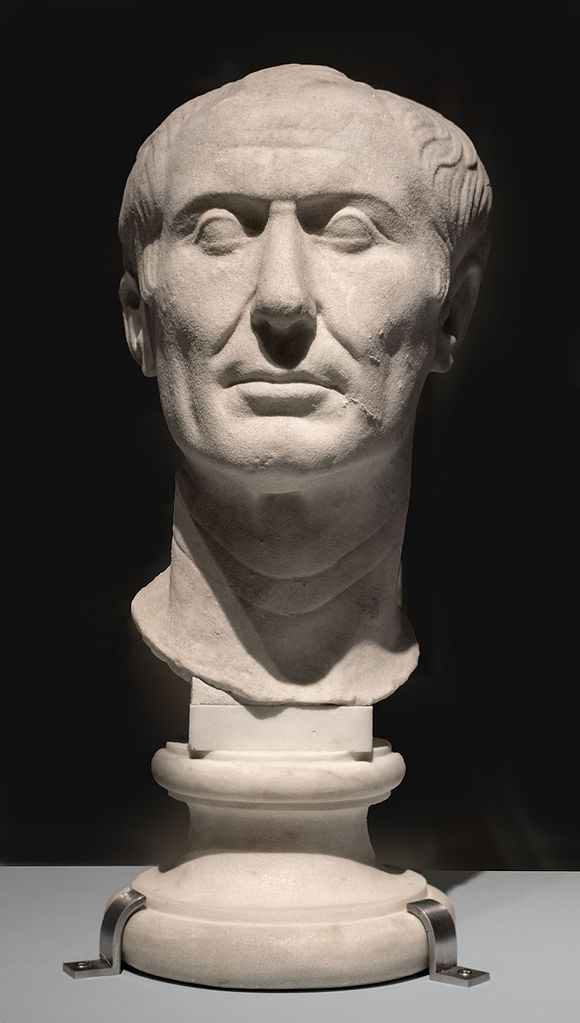
\includegraphics[width=0.5\textwidth]{figures/ceasar.jpg}\\
				\hspace*{15pt}\hbox{\scriptsize Image By:\thinspace{\itshape Ángel M. Felicísimo}}
				%https://commons.wikimedia.org/wiki/File:Retrato_de_Julio_C%C3%A9sar_(26724093101).jpg
			\end{center}

			\column{0.455\textwidth}
			\begin{center}
				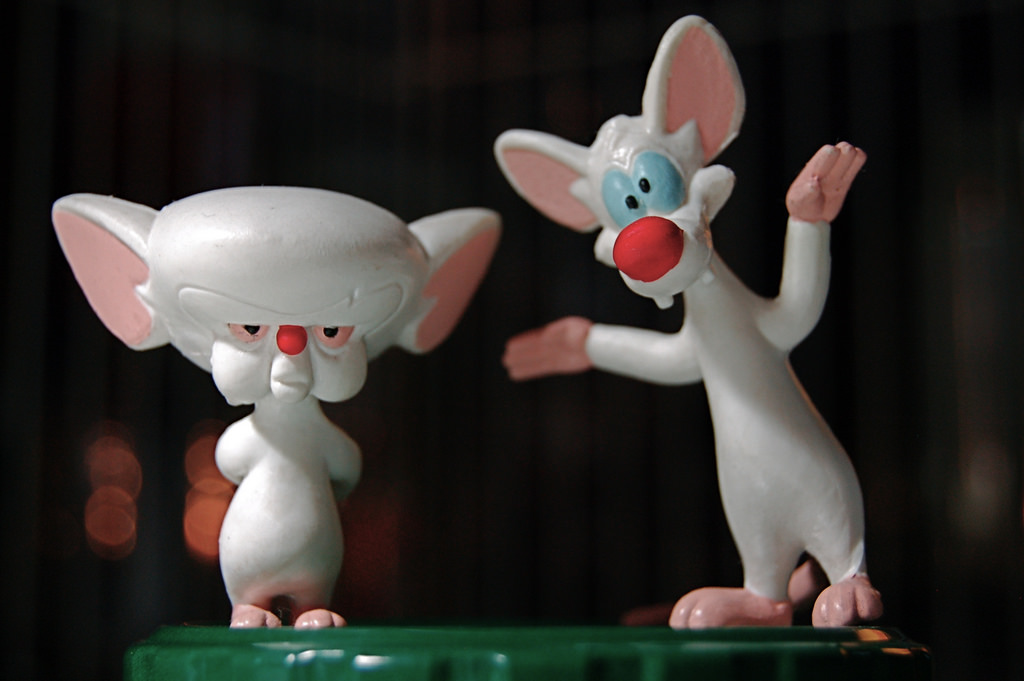
\includegraphics[width=0.9\textwidth]{figures/pinky.jpg}\\
				\hspace*{15pt}\hbox{\scriptsize Image By:\thinspace{\itshape JD Hancock}}
				%https://commons.wikimedia.org/wiki/File:Retrato_de_Julio_C%C3%A9sar_(26724093101).jpg

			\end{center}
		\end{columns}
\end{frame}

\begin{frame}
	\frametitle{Ideas for an algorithm}

	\begin{overlayarea}{\textwidth}{\textheight}
		\input{figures/tikz/closestpair_fixed.tex}
		
		\pause
		\begin{exampleblock}{Algorithm}
			\begin{itemize}
				\item \alert<2>{Divide}: Draw vertical line $L$ that has roughly half of the points on each side.
					\pause
				\item \alert<3>{Conquer}: Find the closest pair on each side.
					\pause
				\item \alert<4>{Combine}: Find the closest pair with one point on each side.
					\pause
				\item Return the minimum of these 3.
			\end{itemize}
		\end{exampleblock}	
	\end{overlayarea}
\end{frame}

\begin{frame}
	\frametitle{Did we make things better?}
	\begin{questionblock}{What is the run time of combine?}
		How much time to combine the two halves? Remember that we want to improve over $\Theta(n^2)$.
	\end{questionblock}	
\end{frame}

\begin{frame}
	\frametitle{How do we make it better?}
		\input{figures/tikz/closestpair_fixed2.tex}
	Observation:
	\begin{itemize}
		\item If $\delta$ is the minimum of the smallest distances left and right.
			\pause
		\item Then we only need to consider pairs of points within $\delta$ of $L$.
			\pause
		\item So in this example, none at all!
	\end{itemize}
\end{frame}

\begin{frame}
	\frametitle{Worst-case?}
	\begin{overlayarea}{\textwidth}{\textheight}
			\begin{itemize}
				\item But worst-case all points are in this $2\delta$-strip...
					\pause
				\item But if we sort them by $y$-coordinate (which can be done in $O(n\log n)$), then how many comparisons do we need?
					\pause
				\item Still $O(n^2)$!?
					\only<4->{
				\item Nope! We only need to check within 11 (i.e. a constant number of) positions in the sorted list.
				}
					\only<5->{
				\item So the combining step is $O(n \log n)$ (which can be further improved to $O(n)$)!
				}
			\end{itemize}
			\only<3>{
			\begin{center}
				
\includegraphics[width=0.4\textwidth]{figures/dilbert.jpg}
				\framesubtitle{http://thecontextofthings.com/wp-content/uploads/2017/11/dilbert-work.jpg}
			\end{center}
		}
	\end{overlayarea}
\end{frame}

\begin{frame}
	\frametitle{Why 11?}

	\begin{overlayarea}{\textwidth}{\textheight}
		\begin{columns}
			\column{0.655\textwidth}
			\begin{block}{Definition}
				Let $s_i$ be the point in the $2\delta$-strip with the $i^\text{th}$ smallest $y$-coordinate.
			\end{block}	
			
			\pause
			\begin{block}{Claim about 11}
				If $|i-j| > 11$ then the distance between $s_i$ and $s_j$ is at least $\delta$.
			\end{block}
			\column{0.255\textwidth}
			\input{figures/tikz/closestpair_delta.tex}	
		\end{columns}
		
		\pause
		\only<3-5>{
			\begin{block}{Proof sketch}
			\begin{itemize}
				\item No two points are in the same $0.5\delta$-by-$0.5\delta$-box.
					\only<4->{
				\item Two points that have two rows between them have a distance $\geq 2\cdot(0.5\delta) = \delta$.
				}
				\only<5->{
				\item So we only consider points at most 2 rows away.
				}
			\end{itemize}
		\end{block}
	}
	\only<6->{
		\begin{exampleblock}{Fun facts!}
			\begin{itemize}
				\item We can even reduce this to just 7 points.
					\only<7>{
				\item Even less if we consider columns separately.
				}
			\end{itemize}
		\end{exampleblock}	
	}
		
		\only<3>{
		\begin{questionblock}{Why not?}
			Why are there no two points in the same box?
		\end{questionblock}
}
	\end{overlayarea}
\end{frame}

\begin{frame}
	\frametitle{The algorithm}
	\begin{columns}
		\column{0.705\textwidth}
	\begin{algorithmic}
		\State Sort all points by x-coordinate
		\Function{Closest-Pair}{$p_1,\dots,p_n$}
			\If{n=1}
				\State \Return $\infty$
			\EndIf

			\pause
			\State $L \gets$ \alert<2>{median} $x$-coordinate
			\State $\delta_1 \gets$ \Call{Closest-Pair}{Points left of $L$}
			\State $\delta_2 \gets$ \Call{Closest-Pair}{Points right of $L$}
			\State $\delta \gets \min(\delta_1,\delta_2)$
			\pause
			\State get list of all points within $\delta$ from L.
			\State sort this list by y-coordinate
			\pause
			\State Scan by y-order, compare every point to the next 11 and update $\delta$ as you go.
			\State \Return $\delta$
		\EndFunction
	\end{algorithmic}
		\pnote{Why not the average?}
		\column{0.205\textwidth}
		\pause
		\begin{questionblock}{}
			What is the recurrence equation for the run time?	
		\end{questionblock}	
		\pause
		\begin{answerblock}{}
			\small
			$T(n) =2T(n/2) + O(n\log n)$	
		\end{answerblock}
	\end{columns}
	
\end{frame}

		\begin{questionblock}{Brute-force}
			What is the tightest upper bound on the run time for a brute-force solution given $|S| = n$?
			\only<2>{
			\begin{enumerate}[A.]
				\item $O(n \log n)$
				\item $O(n^2)$
				\item $O(n^2 \log n)$
				\item $O(n^3)$
				\item I don't know.
			\end{enumerate}
		}
		\end{questionblock}
		\only<3>{
			\begin{answerblock}{Try every combination}
				We check every pair of points, of which there are $n^2$, so $O(n^2)$.	
			\end{answerblock}
		}
	\end{overlayarea}
\end{frame}

\begin{frame}
	\frametitle{Time to improve!}
	\framesubtitle{Using Divide \& Conquer}
		\begin{columns}
			\column{0.455\textwidth}
			\begin{center}
				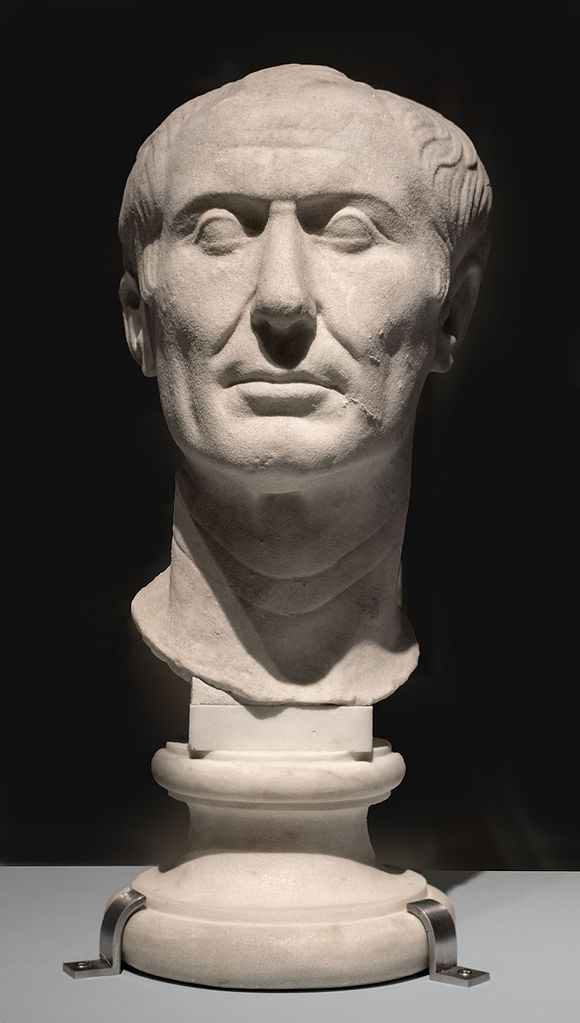
\includegraphics[width=0.5\textwidth]{figures/ceasar.jpg}\\
				\hspace*{15pt}\hbox{\scriptsize Image By:\thinspace{\itshape Ángel M. Felicísimo}}
				%https://commons.wikimedia.org/wiki/File:Retrato_de_Julio_C%C3%A9sar_(26724093101).jpg
			\end{center}

			\column{0.455\textwidth}
			\begin{center}
				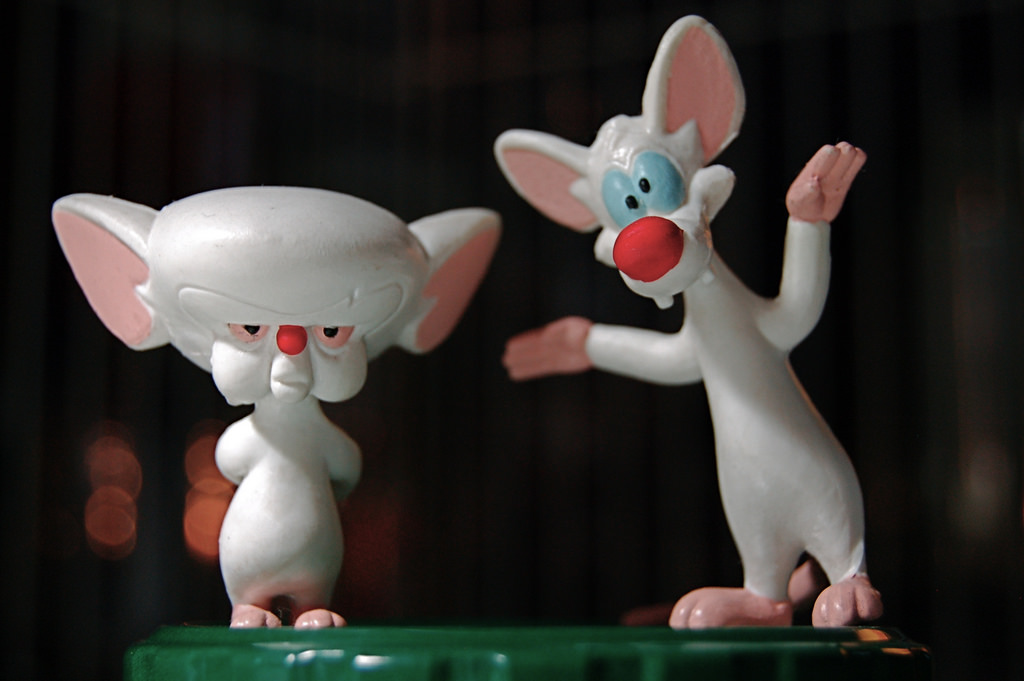
\includegraphics[width=0.9\textwidth]{figures/pinky.jpg}\\
				\hspace*{15pt}\hbox{\scriptsize Image By:\thinspace{\itshape JD Hancock}}
				%https://commons.wikimedia.org/wiki/File:Retrato_de_Julio_C%C3%A9sar_(26724093101).jpg

			\end{center}
		\end{columns}
\end{frame}

\begin{frame}
	\frametitle{Ideas for an algorithm}

	\begin{overlayarea}{\textwidth}{\textheight}
		\begin{figure}[htpb]
\begin{center}
\begin{tikzpicture}[scale=0.5, transform shape]
	\draw (-8,-3) rectangle (8,3);

	\foreach \x/\y/\name in {
		-7/2/,
		-6/1/l1,
		-5/1/l2,
		-3/-2/c1,
		-1/-2/c2,
		3/-1/,
		5/1.5/r1,
		5/0/r2,
		}{
		\node[circle, black, draw, fill=blue!30, minimum size=4pt] (\name) at (\x,\y) {};
	}
		\node at (-1.5, -3.5) {};
	\only<2->{
		\draw[dotted] (-1.5,-3) -- (-1.5,3);
		\node at (-1.5, -3.5) {\Large $L$};
	}
	\only<3->{
		\draw[dotted, red, thick] (l1) --  node[anchor=south] {\Large 1} (l2);
		\draw[dotted, red, thick] (r1) --  node[anchor=west] {\Large 1.5} (r2);
	}
	\only<4->{
		\draw[dotted, red, thick] (c1) --  node[anchor=south] {\Large 2} (c2);
	}
\end{tikzpicture}
\end{center}
\end{figure}

		
		\pause
		\begin{exampleblock}{Algorithm}
			\begin{itemize}
				\item \alert<2>{Divide}: Draw vertical line $L$ that has roughly half of the points on each side.
					\pause
				\item \alert<3>{Conquer}: Find the closest pair on each side.
					\pause
				\item \alert<4>{Combine}: Find the closest pair with one point on each side.
					\pause
				\item Return the minimum of these 3.
			\end{itemize}
		\end{exampleblock}	
	\end{overlayarea}
\end{frame}

\begin{frame}
	\frametitle{Did we make things better?}
	\begin{questionblock}{What is the run time of combine?}
		How much time to combine the two halves? Remember that we want to improve over $\Theta(n^2)$.
	\end{questionblock}	
\end{frame}

\begin{frame}
	\frametitle{How do we make it better?}
		\begin{figure}[htpb]
\begin{center}
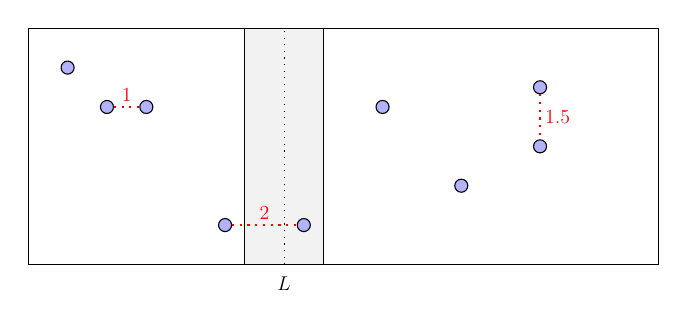
\begin{tikzpicture}[scale=0.5, transform shape]
	\draw (-8,-3) rectangle (8,3);

	\only<2->{
		\draw[fill=gray!10] (-2.5,-3) rectangle (-0.5,3);
	}
	\foreach \x/\y/\name in {
		-7/2/,
		-6/1/l1,
		-5/1/l2,
		-3/-2/c1,
		-1/-2/c2,
		3/-1/,
		5/1.5/r1,
		5/0/r2,
		}{
		\node[circle, black, draw, fill=blue!30, minimum size=4pt] (\name) at (\x,\y) {};
	}
		\draw[dotted] (-1.5,-3) -- (-1.5,3);
		\node at (-1.5, -3.5) {\Large $L$};
		\draw[dotted, red, thick] (l1) --  node[anchor=south] {\Large 1} (l2);
		\draw[dotted, red, thick] (r1) --  node[anchor=west] {\Large 1.5} (r2);
		\draw[dotted, red, thick] (c1) --  node[anchor=south] {\Large 2} (c2);

\end{tikzpicture}
\end{center}
\end{figure}

	Observation:
	\begin{itemize}
		\item If $\delta$ is the minimum of the smallest distances left and right.
			\pause
		\item Then we only need to consider pairs of points within $\delta$ of $L$.
			\pause
		\item So in this example, none at all!
	\end{itemize}
\end{frame}

\begin{frame}
	\frametitle{Worst-case?}
	\begin{overlayarea}{\textwidth}{\textheight}
			\begin{itemize}
				\item But worst-case all points are in this $2\delta$-strip...
					\pause
				\item But if we sort them by $y$-coordinate (which can be done in $O(n\log n)$), then how many comparisons do we need?
					\pause
				\item Still $O(n^2)$!?
					\only<4->{
				\item Nope! We only need to check within 11 (i.e. a constant number of) positions in the sorted list.
				}
					\only<5->{
				\item So the combining step is $O(n \log n)$ (which can be further improved to $O(n)$)!
				}
			\end{itemize}
			\only<3>{
			\begin{center}
				
\includegraphics[width=0.4\textwidth]{figures/dilbert.jpg}
				\framesubtitle{http://thecontextofthings.com/wp-content/uploads/2017/11/dilbert-work.jpg}
			\end{center}
		}
	\end{overlayarea}
\end{frame}

\begin{frame}
	\frametitle{Why 11?}

	\begin{overlayarea}{\textwidth}{\textheight}
		\begin{columns}
			\column{0.655\textwidth}
			\begin{block}{Definition}
				Let $s_i$ be the point in the $2\delta$-strip with the $i^\text{th}$ smallest $y$-coordinate.
			\end{block}	
			
			\pause
			\begin{block}{Claim about 11}
				If $|i-j| > 11$ then the distance between $s_i$ and $s_j$ is at least $\delta$.
			\end{block}
			\column{0.255\textwidth}
			\begin{figure}[htpb]
\begin{center}
\begin{tikzpicture}[scale=0.4, transform shape]
	\draw (-2,-4) rectangle (2,4);
	
	\only<5->{
		\foreach \y in {-2, ..., 0}{
			\foreach \x in {-2, ..., 1}{
				\draw[fill=green!30] (\x,\y) rectangle (\x+1,\y+1);
			}
		}
	}

	\foreach \x/\y/\name/\color in {
		1.35/-2.4/1/red,
		-1.35/-1.6/2/green,
		-0.4/-0.4/3/blue,
		1.3/0.5/4/blue,
	%	1.7/1.4/5/red,
		-0.4/2.4/5/red,
		0.3/2.4/6/red}{
		\alt<4->{
		\node[circle, black, draw, fill=\color!30, minimum size=4pt] () at (\x,\y) {\name};
			}{
		\node[circle, black, draw, fill=blue!30, minimum size=4pt] () at (\x,\y) {\name};
		}
	}
		\draw[thick] (0,-4) -- (0,4);
		\node at (0, -4.5) {\Large $L$};
		\node at (-2, -4.5) {\Large $L-\delta$};
		\node at (2, -4.5) {\Large $L+\delta$};
		\only<3->{
			\draw[dotted] (1,-4) -- (1,4);
			\draw[dotted] (-1,-4) -- (-1,4);

			\foreach \y in {-3, ..., 3}{
				\draw[dotted] (-2,\y) -- (2,\y);
			}
		}

\end{tikzpicture}
\end{center}
\end{figure}
	
		\end{columns}
		
		\pause
		\only<3-5>{
			\begin{block}{Proof sketch}
			\begin{itemize}
				\item No two points are in the same $0.5\delta$-by-$0.5\delta$-box.
					\only<4->{
				\item Two points that have two rows between them have a distance $\geq 2\cdot(0.5\delta) = \delta$.
				}
				\only<5->{
				\item So we only consider points at most 2 rows away.
				}
			\end{itemize}
		\end{block}
	}
	\only<6->{
		\begin{exampleblock}{Fun facts!}
			\begin{itemize}
				\item We can even reduce this to just 7 points.
					\only<7>{
				\item Even less if we consider columns separately.
				}
			\end{itemize}
		\end{exampleblock}	
	}
		
		\only<3>{
		\begin{questionblock}{Why not?}
			Why are there no two points in the same box?
		\end{questionblock}
}
	\end{overlayarea}
\end{frame}

\begin{frame}
	\frametitle{The algorithm}
	\begin{columns}
		\column{0.705\textwidth}
	\begin{algorithmic}
		\State Sort all points by x-coordinate
		\Function{Closest-Pair}{$p_1,\dots,p_n$}
			\If{n=1}
				\State \Return $\infty$
			\EndIf

			\pause
			\State $L \gets$ \alert<2>{median} $x$-coordinate
			\State $\delta_1 \gets$ \Call{Closest-Pair}{Points left of $L$}
			\State $\delta_2 \gets$ \Call{Closest-Pair}{Points right of $L$}
			\State $\delta \gets \min(\delta_1,\delta_2)$
			\pause
			\State get list of all points within $\delta$ from L.
			\State sort this list by y-coordinate
			\pause
			\State Scan by y-order, compare every point to the next 11 and update $\delta$ as you go.
			\State \Return $\delta$
		\EndFunction
	\end{algorithmic}
		\pnote{Why not the average?}
		\column{0.205\textwidth}
		\pause
		\begin{questionblock}{}
			What is the recurrence equation for the run time?	
		\end{questionblock}	
		\pause
		\begin{answerblock}{}
			\small
			$T(n) =2T(n/2) + O(n\log n)$	
		\end{answerblock}
	\end{columns}
	
\end{frame}

	\pnote{Why is this relevant? Answers: For instance collision detection algorithms}
\end{frame}

\begin{frame}
	\frametitle{Let's just brute-force it?}
	\begin{overlayarea}{\textwidth}{\textheight}
		\section{Closest pair of points}
\label{sec:closest_pair_of_points}


\begin{frame}
	\frametitle{A new problem}
	\begin{problemblock}{Closest pair of points}
		Given a set of points, what is the pair of points that is closest to each other?\\
		\pause
		More formally:
		\begin{itemize}
			\item Given a set of points $S$, where every point $p_i$ has an x-coordinate $x_i$ and y-coordinate $y_i$.
			\item Distance is defined as: $d(i,j) = \sqrt{{(x_i - x_j)}^{2} + {(y_i-y_j)}^2}$
			\item What is the pair of points $i,j$ such that $d(i,j)$ is minimal?
		\end{itemize}
	\end{problemblock}
	\pause
	\section{Closest pair of points}
\label{sec:closest_pair_of_points}


\begin{frame}
	\frametitle{A new problem}
	\begin{problemblock}{Closest pair of points}
		Given a set of points, what is the pair of points that is closest to each other?\\
		\pause
		More formally:
		\begin{itemize}
			\item Given a set of points $S$, where every point $p_i$ has an x-coordinate $x_i$ and y-coordinate $y_i$.
			\item Distance is defined as: $d(i,j) = \sqrt{{(x_i - x_j)}^{2} + {(y_i-y_j)}^2}$
			\item What is the pair of points $i,j$ such that $d(i,j)$ is minimal?
		\end{itemize}
	\end{problemblock}
	\pause
	\input{figures/tikz/closestpair.tex}
	\pnote{Why is this relevant? Answers: For instance collision detection algorithms}
\end{frame}

\begin{frame}
	\frametitle{Let's just brute-force it?}
	\begin{overlayarea}{\textwidth}{\textheight}
		\input{figures/tikz/closestpair.tex}
		\begin{questionblock}{Brute-force}
			What is the tightest upper bound on the run time for a brute-force solution given $|S| = n$?
			\only<2>{
			\begin{enumerate}[A.]
				\item $O(n \log n)$
				\item $O(n^2)$
				\item $O(n^2 \log n)$
				\item $O(n^3)$
				\item I don't know.
			\end{enumerate}
		}
		\end{questionblock}
		\only<3>{
			\begin{answerblock}{Try every combination}
				We check every pair of points, of which there are $n^2$, so $O(n^2)$.	
			\end{answerblock}
		}
	\end{overlayarea}
\end{frame}

\begin{frame}
	\frametitle{Time to improve!}
	\framesubtitle{Using Divide \& Conquer}
		\begin{columns}
			\column{0.455\textwidth}
			\begin{center}
				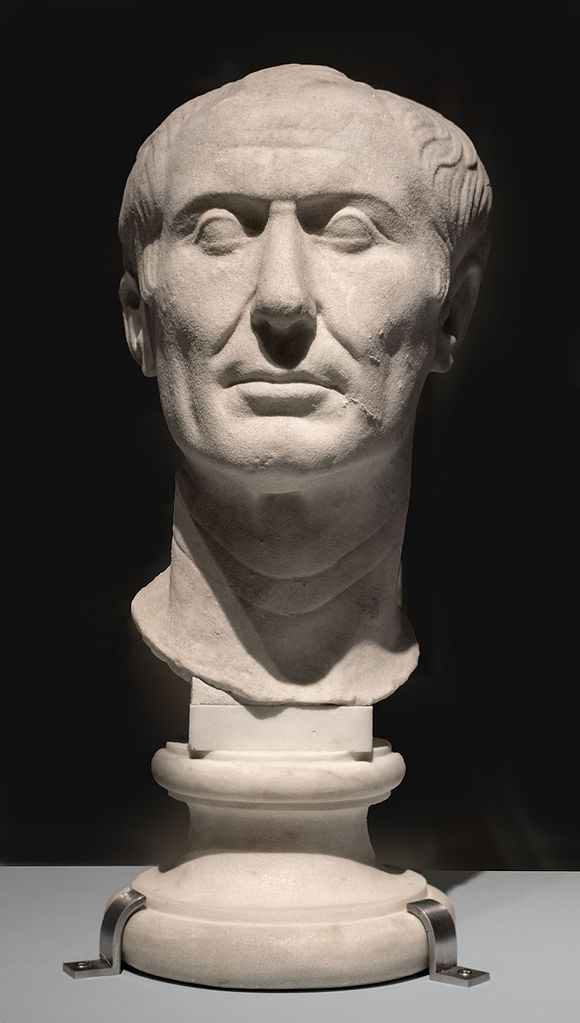
\includegraphics[width=0.5\textwidth]{figures/ceasar.jpg}\\
				\hspace*{15pt}\hbox{\scriptsize Image By:\thinspace{\itshape Ángel M. Felicísimo}}
				%https://commons.wikimedia.org/wiki/File:Retrato_de_Julio_C%C3%A9sar_(26724093101).jpg
			\end{center}

			\column{0.455\textwidth}
			\begin{center}
				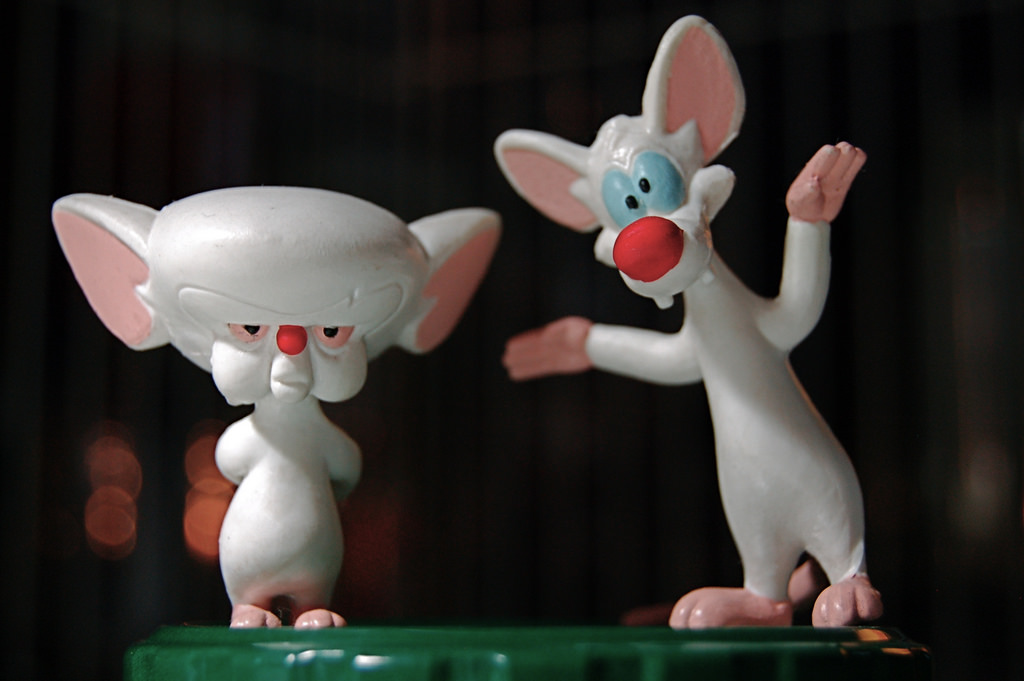
\includegraphics[width=0.9\textwidth]{figures/pinky.jpg}\\
				\hspace*{15pt}\hbox{\scriptsize Image By:\thinspace{\itshape JD Hancock}}
				%https://commons.wikimedia.org/wiki/File:Retrato_de_Julio_C%C3%A9sar_(26724093101).jpg

			\end{center}
		\end{columns}
\end{frame}

\begin{frame}
	\frametitle{Ideas for an algorithm}

	\begin{overlayarea}{\textwidth}{\textheight}
		\input{figures/tikz/closestpair_fixed.tex}
		
		\pause
		\begin{exampleblock}{Algorithm}
			\begin{itemize}
				\item \alert<2>{Divide}: Draw vertical line $L$ that has roughly half of the points on each side.
					\pause
				\item \alert<3>{Conquer}: Find the closest pair on each side.
					\pause
				\item \alert<4>{Combine}: Find the closest pair with one point on each side.
					\pause
				\item Return the minimum of these 3.
			\end{itemize}
		\end{exampleblock}	
	\end{overlayarea}
\end{frame}

\begin{frame}
	\frametitle{Did we make things better?}
	\begin{questionblock}{What is the run time of combine?}
		How much time to combine the two halves? Remember that we want to improve over $\Theta(n^2)$.
	\end{questionblock}	
\end{frame}

\begin{frame}
	\frametitle{How do we make it better?}
		\input{figures/tikz/closestpair_fixed2.tex}
	Observation:
	\begin{itemize}
		\item If $\delta$ is the minimum of the smallest distances left and right.
			\pause
		\item Then we only need to consider pairs of points within $\delta$ of $L$.
			\pause
		\item So in this example, none at all!
	\end{itemize}
\end{frame}

\begin{frame}
	\frametitle{Worst-case?}
	\begin{overlayarea}{\textwidth}{\textheight}
			\begin{itemize}
				\item But worst-case all points are in this $2\delta$-strip...
					\pause
				\item But if we sort them by $y$-coordinate (which can be done in $O(n\log n)$), then how many comparisons do we need?
					\pause
				\item Still $O(n^2)$!?
					\only<4->{
				\item Nope! We only need to check within 11 (i.e. a constant number of) positions in the sorted list.
				}
					\only<5->{
				\item So the combining step is $O(n \log n)$ (which can be further improved to $O(n)$)!
				}
			\end{itemize}
			\only<3>{
			\begin{center}
				
\includegraphics[width=0.4\textwidth]{figures/dilbert.jpg}
				\framesubtitle{http://thecontextofthings.com/wp-content/uploads/2017/11/dilbert-work.jpg}
			\end{center}
		}
	\end{overlayarea}
\end{frame}

\begin{frame}
	\frametitle{Why 11?}

	\begin{overlayarea}{\textwidth}{\textheight}
		\begin{columns}
			\column{0.655\textwidth}
			\begin{block}{Definition}
				Let $s_i$ be the point in the $2\delta$-strip with the $i^\text{th}$ smallest $y$-coordinate.
			\end{block}	
			
			\pause
			\begin{block}{Claim about 11}
				If $|i-j| > 11$ then the distance between $s_i$ and $s_j$ is at least $\delta$.
			\end{block}
			\column{0.255\textwidth}
			\input{figures/tikz/closestpair_delta.tex}	
		\end{columns}
		
		\pause
		\only<3-5>{
			\begin{block}{Proof sketch}
			\begin{itemize}
				\item No two points are in the same $0.5\delta$-by-$0.5\delta$-box.
					\only<4->{
				\item Two points that have two rows between them have a distance $\geq 2\cdot(0.5\delta) = \delta$.
				}
				\only<5->{
				\item So we only consider points at most 2 rows away.
				}
			\end{itemize}
		\end{block}
	}
	\only<6->{
		\begin{exampleblock}{Fun facts!}
			\begin{itemize}
				\item We can even reduce this to just 7 points.
					\only<7>{
				\item Even less if we consider columns separately.
				}
			\end{itemize}
		\end{exampleblock}	
	}
		
		\only<3>{
		\begin{questionblock}{Why not?}
			Why are there no two points in the same box?
		\end{questionblock}
}
	\end{overlayarea}
\end{frame}

\begin{frame}
	\frametitle{The algorithm}
	\begin{columns}
		\column{0.705\textwidth}
	\begin{algorithmic}
		\State Sort all points by x-coordinate
		\Function{Closest-Pair}{$p_1,\dots,p_n$}
			\If{n=1}
				\State \Return $\infty$
			\EndIf

			\pause
			\State $L \gets$ \alert<2>{median} $x$-coordinate
			\State $\delta_1 \gets$ \Call{Closest-Pair}{Points left of $L$}
			\State $\delta_2 \gets$ \Call{Closest-Pair}{Points right of $L$}
			\State $\delta \gets \min(\delta_1,\delta_2)$
			\pause
			\State get list of all points within $\delta$ from L.
			\State sort this list by y-coordinate
			\pause
			\State Scan by y-order, compare every point to the next 11 and update $\delta$ as you go.
			\State \Return $\delta$
		\EndFunction
	\end{algorithmic}
		\pnote{Why not the average?}
		\column{0.205\textwidth}
		\pause
		\begin{questionblock}{}
			What is the recurrence equation for the run time?	
		\end{questionblock}	
		\pause
		\begin{answerblock}{}
			\small
			$T(n) =2T(n/2) + O(n\log n)$	
		\end{answerblock}
	\end{columns}
	
\end{frame}

	\pnote{Why is this relevant? Answers: For instance collision detection algorithms}
\end{frame}

\begin{frame}
	\frametitle{Let's just brute-force it?}
	\begin{overlayarea}{\textwidth}{\textheight}
		\section{Closest pair of points}
\label{sec:closest_pair_of_points}


\begin{frame}
	\frametitle{A new problem}
	\begin{problemblock}{Closest pair of points}
		Given a set of points, what is the pair of points that is closest to each other?\\
		\pause
		More formally:
		\begin{itemize}
			\item Given a set of points $S$, where every point $p_i$ has an x-coordinate $x_i$ and y-coordinate $y_i$.
			\item Distance is defined as: $d(i,j) = \sqrt{{(x_i - x_j)}^{2} + {(y_i-y_j)}^2}$
			\item What is the pair of points $i,j$ such that $d(i,j)$ is minimal?
		\end{itemize}
	\end{problemblock}
	\pause
	\input{figures/tikz/closestpair.tex}
	\pnote{Why is this relevant? Answers: For instance collision detection algorithms}
\end{frame}

\begin{frame}
	\frametitle{Let's just brute-force it?}
	\begin{overlayarea}{\textwidth}{\textheight}
		\input{figures/tikz/closestpair.tex}
		\begin{questionblock}{Brute-force}
			What is the tightest upper bound on the run time for a brute-force solution given $|S| = n$?
			\only<2>{
			\begin{enumerate}[A.]
				\item $O(n \log n)$
				\item $O(n^2)$
				\item $O(n^2 \log n)$
				\item $O(n^3)$
				\item I don't know.
			\end{enumerate}
		}
		\end{questionblock}
		\only<3>{
			\begin{answerblock}{Try every combination}
				We check every pair of points, of which there are $n^2$, so $O(n^2)$.	
			\end{answerblock}
		}
	\end{overlayarea}
\end{frame}

\begin{frame}
	\frametitle{Time to improve!}
	\framesubtitle{Using Divide \& Conquer}
		\begin{columns}
			\column{0.455\textwidth}
			\begin{center}
				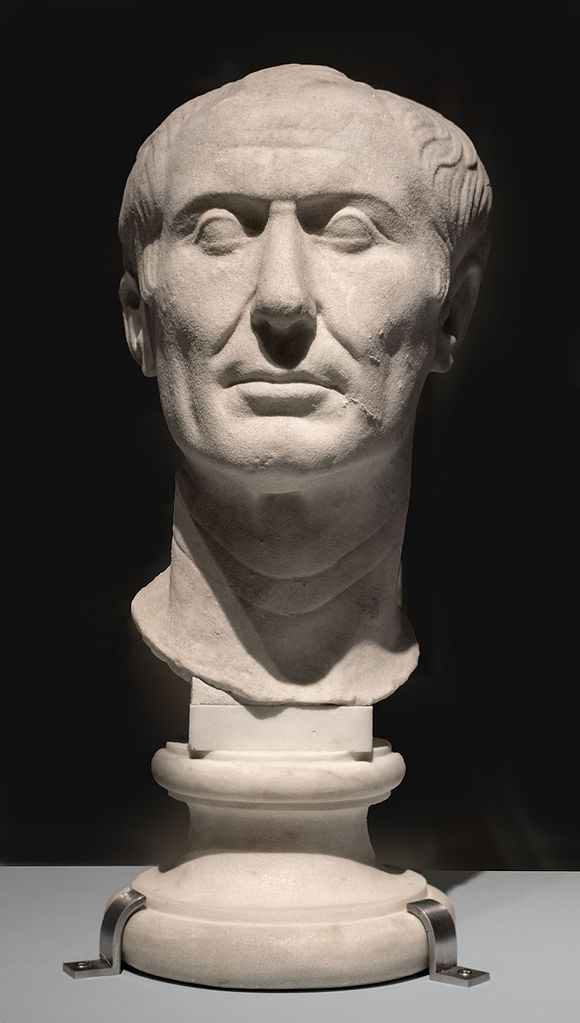
\includegraphics[width=0.5\textwidth]{figures/ceasar.jpg}\\
				\hspace*{15pt}\hbox{\scriptsize Image By:\thinspace{\itshape Ángel M. Felicísimo}}
				%https://commons.wikimedia.org/wiki/File:Retrato_de_Julio_C%C3%A9sar_(26724093101).jpg
			\end{center}

			\column{0.455\textwidth}
			\begin{center}
				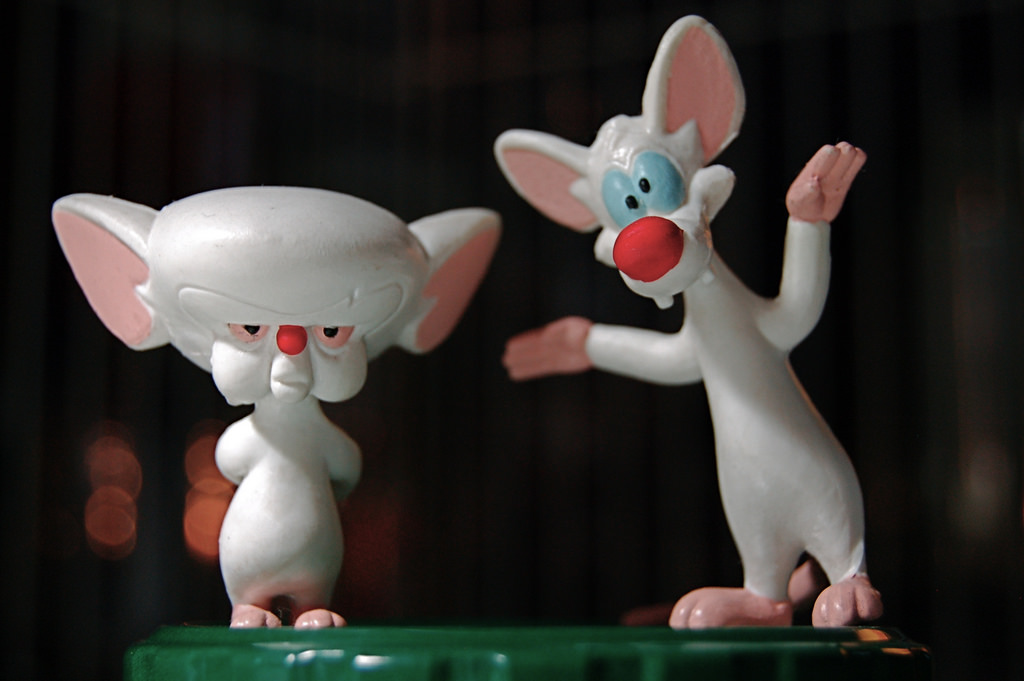
\includegraphics[width=0.9\textwidth]{figures/pinky.jpg}\\
				\hspace*{15pt}\hbox{\scriptsize Image By:\thinspace{\itshape JD Hancock}}
				%https://commons.wikimedia.org/wiki/File:Retrato_de_Julio_C%C3%A9sar_(26724093101).jpg

			\end{center}
		\end{columns}
\end{frame}

\begin{frame}
	\frametitle{Ideas for an algorithm}

	\begin{overlayarea}{\textwidth}{\textheight}
		\input{figures/tikz/closestpair_fixed.tex}
		
		\pause
		\begin{exampleblock}{Algorithm}
			\begin{itemize}
				\item \alert<2>{Divide}: Draw vertical line $L$ that has roughly half of the points on each side.
					\pause
				\item \alert<3>{Conquer}: Find the closest pair on each side.
					\pause
				\item \alert<4>{Combine}: Find the closest pair with one point on each side.
					\pause
				\item Return the minimum of these 3.
			\end{itemize}
		\end{exampleblock}	
	\end{overlayarea}
\end{frame}

\begin{frame}
	\frametitle{Did we make things better?}
	\begin{questionblock}{What is the run time of combine?}
		How much time to combine the two halves? Remember that we want to improve over $\Theta(n^2)$.
	\end{questionblock}	
\end{frame}

\begin{frame}
	\frametitle{How do we make it better?}
		\input{figures/tikz/closestpair_fixed2.tex}
	Observation:
	\begin{itemize}
		\item If $\delta$ is the minimum of the smallest distances left and right.
			\pause
		\item Then we only need to consider pairs of points within $\delta$ of $L$.
			\pause
		\item So in this example, none at all!
	\end{itemize}
\end{frame}

\begin{frame}
	\frametitle{Worst-case?}
	\begin{overlayarea}{\textwidth}{\textheight}
			\begin{itemize}
				\item But worst-case all points are in this $2\delta$-strip...
					\pause
				\item But if we sort them by $y$-coordinate (which can be done in $O(n\log n)$), then how many comparisons do we need?
					\pause
				\item Still $O(n^2)$!?
					\only<4->{
				\item Nope! We only need to check within 11 (i.e. a constant number of) positions in the sorted list.
				}
					\only<5->{
				\item So the combining step is $O(n \log n)$ (which can be further improved to $O(n)$)!
				}
			\end{itemize}
			\only<3>{
			\begin{center}
				
\includegraphics[width=0.4\textwidth]{figures/dilbert.jpg}
				\framesubtitle{http://thecontextofthings.com/wp-content/uploads/2017/11/dilbert-work.jpg}
			\end{center}
		}
	\end{overlayarea}
\end{frame}

\begin{frame}
	\frametitle{Why 11?}

	\begin{overlayarea}{\textwidth}{\textheight}
		\begin{columns}
			\column{0.655\textwidth}
			\begin{block}{Definition}
				Let $s_i$ be the point in the $2\delta$-strip with the $i^\text{th}$ smallest $y$-coordinate.
			\end{block}	
			
			\pause
			\begin{block}{Claim about 11}
				If $|i-j| > 11$ then the distance between $s_i$ and $s_j$ is at least $\delta$.
			\end{block}
			\column{0.255\textwidth}
			\input{figures/tikz/closestpair_delta.tex}	
		\end{columns}
		
		\pause
		\only<3-5>{
			\begin{block}{Proof sketch}
			\begin{itemize}
				\item No two points are in the same $0.5\delta$-by-$0.5\delta$-box.
					\only<4->{
				\item Two points that have two rows between them have a distance $\geq 2\cdot(0.5\delta) = \delta$.
				}
				\only<5->{
				\item So we only consider points at most 2 rows away.
				}
			\end{itemize}
		\end{block}
	}
	\only<6->{
		\begin{exampleblock}{Fun facts!}
			\begin{itemize}
				\item We can even reduce this to just 7 points.
					\only<7>{
				\item Even less if we consider columns separately.
				}
			\end{itemize}
		\end{exampleblock}	
	}
		
		\only<3>{
		\begin{questionblock}{Why not?}
			Why are there no two points in the same box?
		\end{questionblock}
}
	\end{overlayarea}
\end{frame}

\begin{frame}
	\frametitle{The algorithm}
	\begin{columns}
		\column{0.705\textwidth}
	\begin{algorithmic}
		\State Sort all points by x-coordinate
		\Function{Closest-Pair}{$p_1,\dots,p_n$}
			\If{n=1}
				\State \Return $\infty$
			\EndIf

			\pause
			\State $L \gets$ \alert<2>{median} $x$-coordinate
			\State $\delta_1 \gets$ \Call{Closest-Pair}{Points left of $L$}
			\State $\delta_2 \gets$ \Call{Closest-Pair}{Points right of $L$}
			\State $\delta \gets \min(\delta_1,\delta_2)$
			\pause
			\State get list of all points within $\delta$ from L.
			\State sort this list by y-coordinate
			\pause
			\State Scan by y-order, compare every point to the next 11 and update $\delta$ as you go.
			\State \Return $\delta$
		\EndFunction
	\end{algorithmic}
		\pnote{Why not the average?}
		\column{0.205\textwidth}
		\pause
		\begin{questionblock}{}
			What is the recurrence equation for the run time?	
		\end{questionblock}	
		\pause
		\begin{answerblock}{}
			\small
			$T(n) =2T(n/2) + O(n\log n)$	
		\end{answerblock}
	\end{columns}
	
\end{frame}

		\begin{questionblock}{Brute-force}
			What is the tightest upper bound on the run time for a brute-force solution given $|S| = n$?
			\only<2>{
			\begin{enumerate}[A.]
				\item $O(n \log n)$
				\item $O(n^2)$
				\item $O(n^2 \log n)$
				\item $O(n^3)$
				\item I don't know.
			\end{enumerate}
		}
		\end{questionblock}
		\only<3>{
			\begin{answerblock}{Try every combination}
				We check every pair of points, of which there are $n^2$, so $O(n^2)$.	
			\end{answerblock}
		}
	\end{overlayarea}
\end{frame}

\begin{frame}
	\frametitle{Time to improve!}
	\framesubtitle{Using Divide \& Conquer}
		\begin{columns}
			\column{0.455\textwidth}
			\begin{center}
				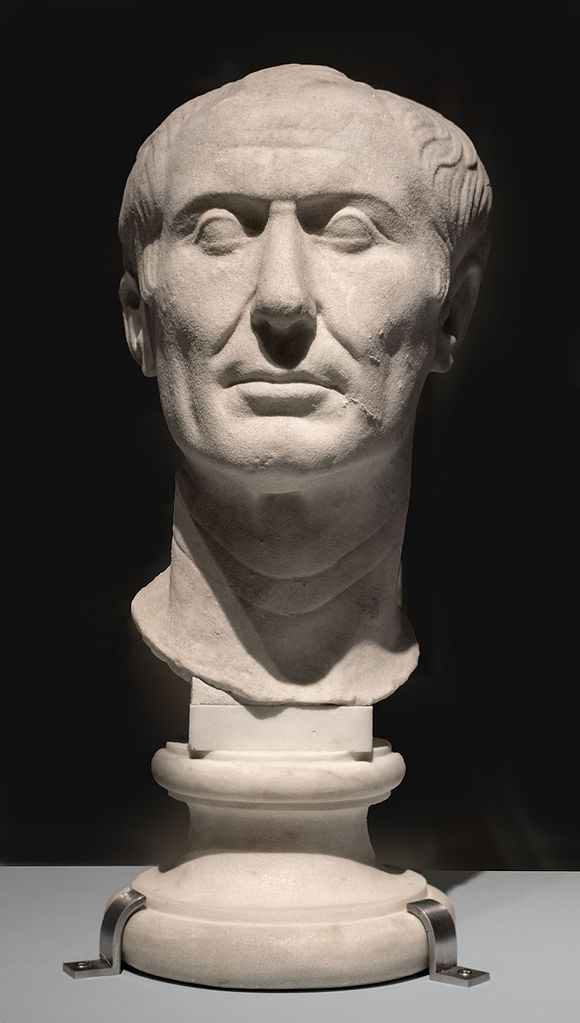
\includegraphics[width=0.5\textwidth]{figures/ceasar.jpg}\\
				\hspace*{15pt}\hbox{\scriptsize Image By:\thinspace{\itshape Ángel M. Felicísimo}}
				%https://commons.wikimedia.org/wiki/File:Retrato_de_Julio_C%C3%A9sar_(26724093101).jpg
			\end{center}

			\column{0.455\textwidth}
			\begin{center}
				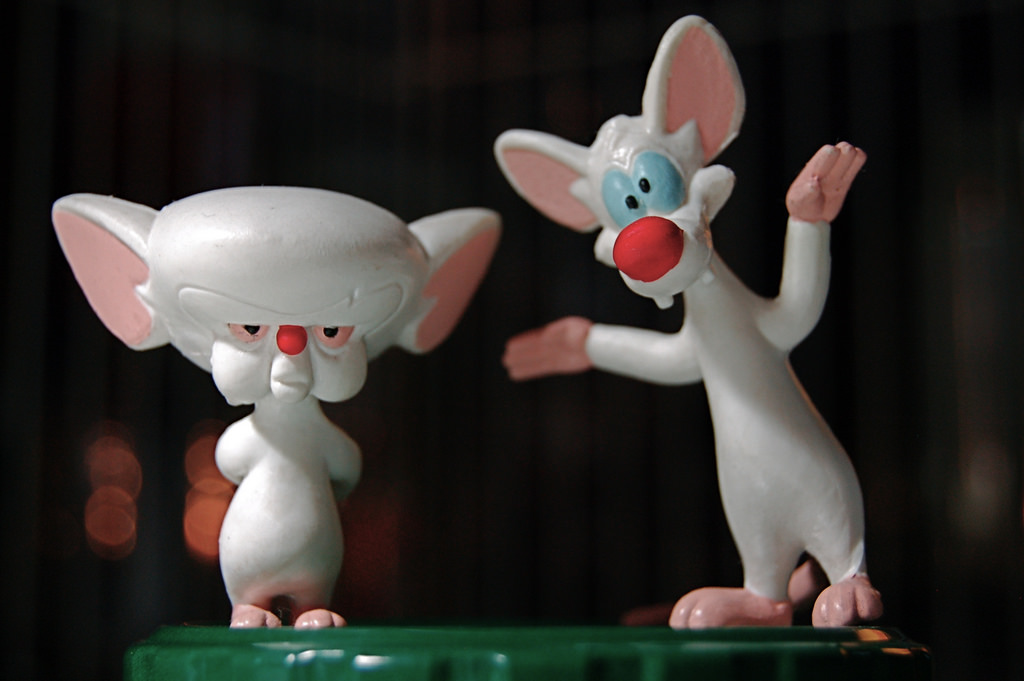
\includegraphics[width=0.9\textwidth]{figures/pinky.jpg}\\
				\hspace*{15pt}\hbox{\scriptsize Image By:\thinspace{\itshape JD Hancock}}
				%https://commons.wikimedia.org/wiki/File:Retrato_de_Julio_C%C3%A9sar_(26724093101).jpg

			\end{center}
		\end{columns}
\end{frame}

\begin{frame}
	\frametitle{Ideas for an algorithm}

	\begin{overlayarea}{\textwidth}{\textheight}
		\begin{figure}[htpb]
\begin{center}
\begin{tikzpicture}[scale=0.5, transform shape]
	\draw (-8,-3) rectangle (8,3);

	\foreach \x/\y/\name in {
		-7/2/,
		-6/1/l1,
		-5/1/l2,
		-3/-2/c1,
		-1/-2/c2,
		3/-1/,
		5/1.5/r1,
		5/0/r2,
		}{
		\node[circle, black, draw, fill=blue!30, minimum size=4pt] (\name) at (\x,\y) {};
	}
		\node at (-1.5, -3.5) {};
	\only<2->{
		\draw[dotted] (-1.5,-3) -- (-1.5,3);
		\node at (-1.5, -3.5) {\Large $L$};
	}
	\only<3->{
		\draw[dotted, red, thick] (l1) --  node[anchor=south] {\Large 1} (l2);
		\draw[dotted, red, thick] (r1) --  node[anchor=west] {\Large 1.5} (r2);
	}
	\only<4->{
		\draw[dotted, red, thick] (c1) --  node[anchor=south] {\Large 2} (c2);
	}
\end{tikzpicture}
\end{center}
\end{figure}

		
		\pause
		\begin{exampleblock}{Algorithm}
			\begin{itemize}
				\item \alert<2>{Divide}: Draw vertical line $L$ that has roughly half of the points on each side.
					\pause
				\item \alert<3>{Conquer}: Find the closest pair on each side.
					\pause
				\item \alert<4>{Combine}: Find the closest pair with one point on each side.
					\pause
				\item Return the minimum of these 3.
			\end{itemize}
		\end{exampleblock}	
	\end{overlayarea}
\end{frame}

\begin{frame}
	\frametitle{Did we make things better?}
	\begin{questionblock}{What is the run time of combine?}
		How much time to combine the two halves? Remember that we want to improve over $\Theta(n^2)$.
	\end{questionblock}	
\end{frame}

\begin{frame}
	\frametitle{How do we make it better?}
		\begin{figure}[htpb]
\begin{center}
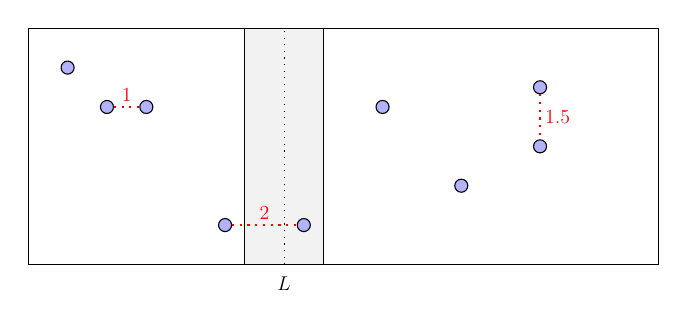
\begin{tikzpicture}[scale=0.5, transform shape]
	\draw (-8,-3) rectangle (8,3);

	\only<2->{
		\draw[fill=gray!10] (-2.5,-3) rectangle (-0.5,3);
	}
	\foreach \x/\y/\name in {
		-7/2/,
		-6/1/l1,
		-5/1/l2,
		-3/-2/c1,
		-1/-2/c2,
		3/-1/,
		5/1.5/r1,
		5/0/r2,
		}{
		\node[circle, black, draw, fill=blue!30, minimum size=4pt] (\name) at (\x,\y) {};
	}
		\draw[dotted] (-1.5,-3) -- (-1.5,3);
		\node at (-1.5, -3.5) {\Large $L$};
		\draw[dotted, red, thick] (l1) --  node[anchor=south] {\Large 1} (l2);
		\draw[dotted, red, thick] (r1) --  node[anchor=west] {\Large 1.5} (r2);
		\draw[dotted, red, thick] (c1) --  node[anchor=south] {\Large 2} (c2);

\end{tikzpicture}
\end{center}
\end{figure}

	Observation:
	\begin{itemize}
		\item If $\delta$ is the minimum of the smallest distances left and right.
			\pause
		\item Then we only need to consider pairs of points within $\delta$ of $L$.
			\pause
		\item So in this example, none at all!
	\end{itemize}
\end{frame}

\begin{frame}
	\frametitle{Worst-case?}
	\begin{overlayarea}{\textwidth}{\textheight}
			\begin{itemize}
				\item But worst-case all points are in this $2\delta$-strip...
					\pause
				\item But if we sort them by $y$-coordinate (which can be done in $O(n\log n)$), then how many comparisons do we need?
					\pause
				\item Still $O(n^2)$!?
					\only<4->{
				\item Nope! We only need to check within 11 (i.e. a constant number of) positions in the sorted list.
				}
					\only<5->{
				\item So the combining step is $O(n \log n)$ (which can be further improved to $O(n)$)!
				}
			\end{itemize}
			\only<3>{
			\begin{center}
				
\includegraphics[width=0.4\textwidth]{figures/dilbert.jpg}
				\framesubtitle{http://thecontextofthings.com/wp-content/uploads/2017/11/dilbert-work.jpg}
			\end{center}
		}
	\end{overlayarea}
\end{frame}

\begin{frame}
	\frametitle{Why 11?}

	\begin{overlayarea}{\textwidth}{\textheight}
		\begin{columns}
			\column{0.655\textwidth}
			\begin{block}{Definition}
				Let $s_i$ be the point in the $2\delta$-strip with the $i^\text{th}$ smallest $y$-coordinate.
			\end{block}	
			
			\pause
			\begin{block}{Claim about 11}
				If $|i-j| > 11$ then the distance between $s_i$ and $s_j$ is at least $\delta$.
			\end{block}
			\column{0.255\textwidth}
			\begin{figure}[htpb]
\begin{center}
\begin{tikzpicture}[scale=0.4, transform shape]
	\draw (-2,-4) rectangle (2,4);
	
	\only<5->{
		\foreach \y in {-2, ..., 0}{
			\foreach \x in {-2, ..., 1}{
				\draw[fill=green!30] (\x,\y) rectangle (\x+1,\y+1);
			}
		}
	}

	\foreach \x/\y/\name/\color in {
		1.35/-2.4/1/red,
		-1.35/-1.6/2/green,
		-0.4/-0.4/3/blue,
		1.3/0.5/4/blue,
	%	1.7/1.4/5/red,
		-0.4/2.4/5/red,
		0.3/2.4/6/red}{
		\alt<4->{
		\node[circle, black, draw, fill=\color!30, minimum size=4pt] () at (\x,\y) {\name};
			}{
		\node[circle, black, draw, fill=blue!30, minimum size=4pt] () at (\x,\y) {\name};
		}
	}
		\draw[thick] (0,-4) -- (0,4);
		\node at (0, -4.5) {\Large $L$};
		\node at (-2, -4.5) {\Large $L-\delta$};
		\node at (2, -4.5) {\Large $L+\delta$};
		\only<3->{
			\draw[dotted] (1,-4) -- (1,4);
			\draw[dotted] (-1,-4) -- (-1,4);

			\foreach \y in {-3, ..., 3}{
				\draw[dotted] (-2,\y) -- (2,\y);
			}
		}

\end{tikzpicture}
\end{center}
\end{figure}
	
		\end{columns}
		
		\pause
		\only<3-5>{
			\begin{block}{Proof sketch}
			\begin{itemize}
				\item No two points are in the same $0.5\delta$-by-$0.5\delta$-box.
					\only<4->{
				\item Two points that have two rows between them have a distance $\geq 2\cdot(0.5\delta) = \delta$.
				}
				\only<5->{
				\item So we only consider points at most 2 rows away.
				}
			\end{itemize}
		\end{block}
	}
	\only<6->{
		\begin{exampleblock}{Fun facts!}
			\begin{itemize}
				\item We can even reduce this to just 7 points.
					\only<7>{
				\item Even less if we consider columns separately.
				}
			\end{itemize}
		\end{exampleblock}	
	}
		
		\only<3>{
		\begin{questionblock}{Why not?}
			Why are there no two points in the same box?
		\end{questionblock}
}
	\end{overlayarea}
\end{frame}

\begin{frame}
	\frametitle{The algorithm}
	\begin{columns}
		\column{0.705\textwidth}
	\begin{algorithmic}
		\State Sort all points by x-coordinate
		\Function{Closest-Pair}{$p_1,\dots,p_n$}
			\If{n=1}
				\State \Return $\infty$
			\EndIf

			\pause
			\State $L \gets$ \alert<2>{median} $x$-coordinate
			\State $\delta_1 \gets$ \Call{Closest-Pair}{Points left of $L$}
			\State $\delta_2 \gets$ \Call{Closest-Pair}{Points right of $L$}
			\State $\delta \gets \min(\delta_1,\delta_2)$
			\pause
			\State get list of all points within $\delta$ from L.
			\State sort this list by y-coordinate
			\pause
			\State Scan by y-order, compare every point to the next 11 and update $\delta$ as you go.
			\State \Return $\delta$
		\EndFunction
	\end{algorithmic}
		\pnote{Why not the average?}
		\column{0.205\textwidth}
		\pause
		\begin{questionblock}{}
			What is the recurrence equation for the run time?	
		\end{questionblock}	
		\pause
		\begin{answerblock}{}
			\small
			$T(n) =2T(n/2) + O(n\log n)$	
		\end{answerblock}
	\end{columns}
	
\end{frame}

		\begin{questionblock}{Brute-force}
			What is the tightest upper bound on the run time for a brute-force solution given $|S| = n$?
			\only<2>{
			\begin{enumerate}[A.]
				\item $O(n \log n)$
				\item $O(n^2)$
				\item $O(n^2 \log n)$
				\item $O(n^3)$
				\item I don't know.
			\end{enumerate}
		}
		\end{questionblock}
		\only<3>{
			\begin{answerblock}{Try every combination}
				We check every pair of points, of which there are $n^2$, so $O(n^2)$.	
			\end{answerblock}
		}
	\end{overlayarea}
\end{frame}

\begin{frame}
	\frametitle{Time to improve!}
	\framesubtitle{Using Divide \& Conquer}
		\begin{columns}
			\column{0.455\textwidth}
			\begin{center}
				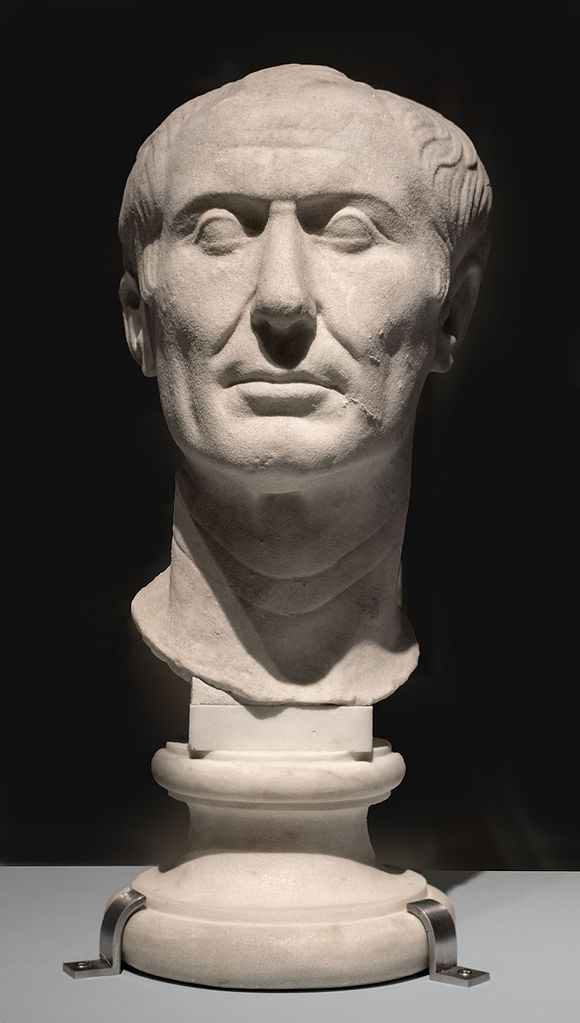
\includegraphics[width=0.5\textwidth]{figures/ceasar.jpg}\\
				\hspace*{15pt}\hbox{\scriptsize Image By:\thinspace{\itshape Ángel M. Felicísimo}}
				%https://commons.wikimedia.org/wiki/File:Retrato_de_Julio_C%C3%A9sar_(26724093101).jpg
			\end{center}

			\column{0.455\textwidth}
			\begin{center}
				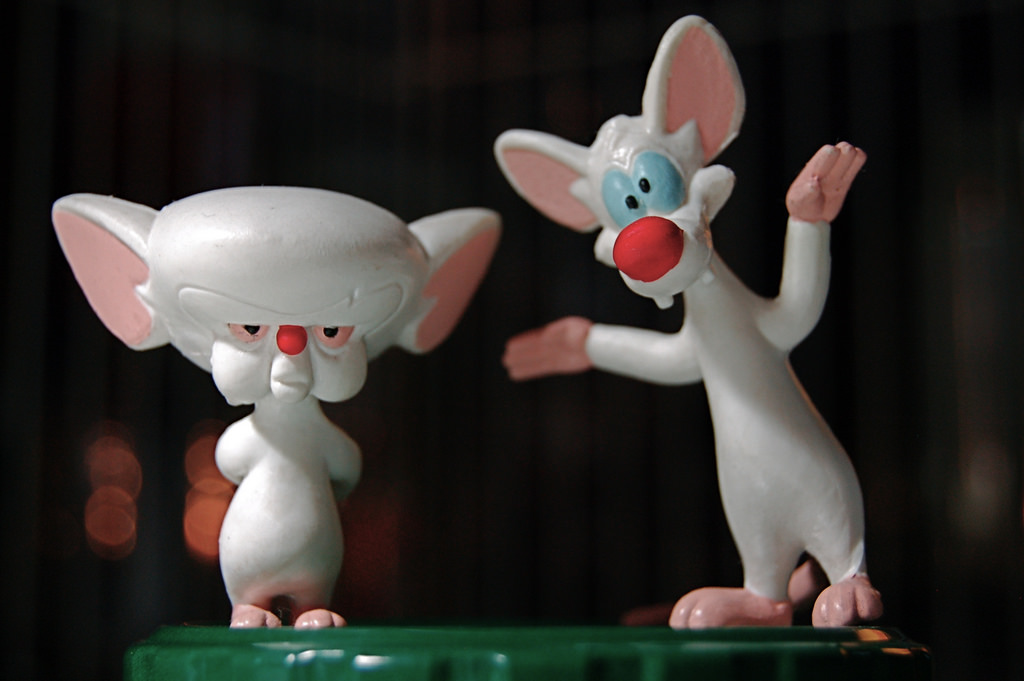
\includegraphics[width=0.9\textwidth]{figures/pinky.jpg}\\
				\hspace*{15pt}\hbox{\scriptsize Image By:\thinspace{\itshape JD Hancock}}
				%https://commons.wikimedia.org/wiki/File:Retrato_de_Julio_C%C3%A9sar_(26724093101).jpg

			\end{center}
		\end{columns}
\end{frame}

\begin{frame}
	\frametitle{Ideas for an algorithm}

	\begin{overlayarea}{\textwidth}{\textheight}
		\begin{figure}[htpb]
\begin{center}
\begin{tikzpicture}[scale=0.5, transform shape]
	\draw (-8,-3) rectangle (8,3);

	\foreach \x/\y/\name in {
		-7/2/,
		-6/1/l1,
		-5/1/l2,
		-3/-2/c1,
		-1/-2/c2,
		3/-1/,
		5/1.5/r1,
		5/0/r2,
		}{
		\node[circle, black, draw, fill=blue!30, minimum size=4pt] (\name) at (\x,\y) {};
	}
		\node at (-1.5, -3.5) {};
	\only<2->{
		\draw[dotted] (-1.5,-3) -- (-1.5,3);
		\node at (-1.5, -3.5) {\Large $L$};
	}
	\only<3->{
		\draw[dotted, red, thick] (l1) --  node[anchor=south] {\Large 1} (l2);
		\draw[dotted, red, thick] (r1) --  node[anchor=west] {\Large 1.5} (r2);
	}
	\only<4->{
		\draw[dotted, red, thick] (c1) --  node[anchor=south] {\Large 2} (c2);
	}
\end{tikzpicture}
\end{center}
\end{figure}

		
		\pause
		\begin{exampleblock}{Algorithm}
			\begin{itemize}
				\item \alert<2>{Divide}: Draw vertical line $L$ that has roughly half of the points on each side.
					\pause
				\item \alert<3>{Conquer}: Find the closest pair on each side.
					\pause
				\item \alert<4>{Combine}: Find the closest pair with one point on each side.
					\pause
				\item Return the minimum of these 3.
			\end{itemize}
		\end{exampleblock}	
	\end{overlayarea}
\end{frame}

\begin{frame}
	\frametitle{Did we make things better?}
	\begin{questionblock}{What is the run time of combine?}
		How much time to combine the two halves? Remember that we want to improve over $\Theta(n^2)$.
	\end{questionblock}	
\end{frame}

\begin{frame}
	\frametitle{How do we make it better?}
		\begin{figure}[htpb]
\begin{center}
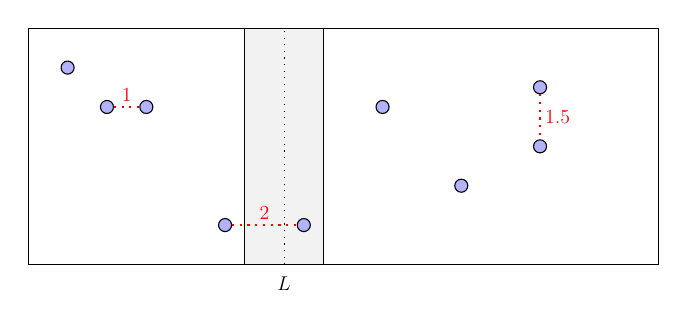
\begin{tikzpicture}[scale=0.5, transform shape]
	\draw (-8,-3) rectangle (8,3);

	\only<2->{
		\draw[fill=gray!10] (-2.5,-3) rectangle (-0.5,3);
	}
	\foreach \x/\y/\name in {
		-7/2/,
		-6/1/l1,
		-5/1/l2,
		-3/-2/c1,
		-1/-2/c2,
		3/-1/,
		5/1.5/r1,
		5/0/r2,
		}{
		\node[circle, black, draw, fill=blue!30, minimum size=4pt] (\name) at (\x,\y) {};
	}
		\draw[dotted] (-1.5,-3) -- (-1.5,3);
		\node at (-1.5, -3.5) {\Large $L$};
		\draw[dotted, red, thick] (l1) --  node[anchor=south] {\Large 1} (l2);
		\draw[dotted, red, thick] (r1) --  node[anchor=west] {\Large 1.5} (r2);
		\draw[dotted, red, thick] (c1) --  node[anchor=south] {\Large 2} (c2);

\end{tikzpicture}
\end{center}
\end{figure}

	Observation:
	\begin{itemize}
		\item If $\delta$ is the minimum of the smallest distances left and right.
			\pause
		\item Then we only need to consider pairs of points within $\delta$ of $L$.
			\pause
		\item So in this example, none at all!
	\end{itemize}
\end{frame}

\begin{frame}
	\frametitle{Worst-case?}
	\begin{overlayarea}{\textwidth}{\textheight}
			\begin{itemize}
				\item But worst-case all points are in this $2\delta$-strip...
					\pause
				\item But if we sort them by $y$-coordinate (which can be done in $O(n\log n)$), then how many comparisons do we need?
					\pause
				\item Still $O(n^2)$!?
					\only<4->{
				\item Nope! We only need to check within 11 (i.e. a constant number of) positions in the sorted list.
				}
					\only<5->{
				\item So the combining step is $O(n \log n)$ (which can be further improved to $O(n)$)!
				}
			\end{itemize}
			\only<3>{
			\begin{center}
				
\includegraphics[width=0.4\textwidth]{figures/dilbert.jpg}
				\framesubtitle{http://thecontextofthings.com/wp-content/uploads/2017/11/dilbert-work.jpg}
			\end{center}
		}
	\end{overlayarea}
\end{frame}

\begin{frame}
	\frametitle{Why 11?}

	\begin{overlayarea}{\textwidth}{\textheight}
		\begin{columns}
			\column{0.655\textwidth}
			\begin{block}{Definition}
				Let $s_i$ be the point in the $2\delta$-strip with the $i^\text{th}$ smallest $y$-coordinate.
			\end{block}	
			
			\pause
			\begin{block}{Claim about 11}
				If $|i-j| > 11$ then the distance between $s_i$ and $s_j$ is at least $\delta$.
			\end{block}
			\column{0.255\textwidth}
			\begin{figure}[htpb]
\begin{center}
\begin{tikzpicture}[scale=0.4, transform shape]
	\draw (-2,-4) rectangle (2,4);
	
	\only<5->{
		\foreach \y in {-2, ..., 0}{
			\foreach \x in {-2, ..., 1}{
				\draw[fill=green!30] (\x,\y) rectangle (\x+1,\y+1);
			}
		}
	}

	\foreach \x/\y/\name/\color in {
		1.35/-2.4/1/red,
		-1.35/-1.6/2/green,
		-0.4/-0.4/3/blue,
		1.3/0.5/4/blue,
	%	1.7/1.4/5/red,
		-0.4/2.4/5/red,
		0.3/2.4/6/red}{
		\alt<4->{
		\node[circle, black, draw, fill=\color!30, minimum size=4pt] () at (\x,\y) {\name};
			}{
		\node[circle, black, draw, fill=blue!30, minimum size=4pt] () at (\x,\y) {\name};
		}
	}
		\draw[thick] (0,-4) -- (0,4);
		\node at (0, -4.5) {\Large $L$};
		\node at (-2, -4.5) {\Large $L-\delta$};
		\node at (2, -4.5) {\Large $L+\delta$};
		\only<3->{
			\draw[dotted] (1,-4) -- (1,4);
			\draw[dotted] (-1,-4) -- (-1,4);

			\foreach \y in {-3, ..., 3}{
				\draw[dotted] (-2,\y) -- (2,\y);
			}
		}

\end{tikzpicture}
\end{center}
\end{figure}
	
		\end{columns}
		
		\pause
		\only<3-5>{
			\begin{block}{Proof sketch}
			\begin{itemize}
				\item No two points are in the same $0.5\delta$-by-$0.5\delta$-box.
					\only<4->{
				\item Two points that have two rows between them have a distance $\geq 2\cdot(0.5\delta) = \delta$.
				}
				\only<5->{
				\item So we only consider points at most 2 rows away.
				}
			\end{itemize}
		\end{block}
	}
	\only<6->{
		\begin{exampleblock}{Fun facts!}
			\begin{itemize}
				\item We can even reduce this to just 7 points.
					\only<7>{
				\item Even less if we consider columns separately.
				}
			\end{itemize}
		\end{exampleblock}	
	}
		
		\only<3>{
		\begin{questionblock}{Why not?}
			Why are there no two points in the same box?
		\end{questionblock}
}
	\end{overlayarea}
\end{frame}

\begin{frame}
	\frametitle{The algorithm}
	\begin{columns}
		\column{0.705\textwidth}
	\begin{algorithmic}
		\State Sort all points by x-coordinate
		\Function{Closest-Pair}{$p_1,\dots,p_n$}
			\If{n=1}
				\State \Return $\infty$
			\EndIf

			\pause
			\State $L \gets$ \alert<2>{median} $x$-coordinate
			\State $\delta_1 \gets$ \Call{Closest-Pair}{Points left of $L$}
			\State $\delta_2 \gets$ \Call{Closest-Pair}{Points right of $L$}
			\State $\delta \gets \min(\delta_1,\delta_2)$
			\pause
			\State get list of all points within $\delta$ from L.
			\State sort this list by y-coordinate
			\pause
			\State Scan by y-order, compare every point to the next 11 and update $\delta$ as you go.
			\State \Return $\delta$
		\EndFunction
	\end{algorithmic}
		\pnote{Why not the average?}
		\column{0.205\textwidth}
		\pause
		\begin{questionblock}{}
			What is the recurrence equation for the run time?	
		\end{questionblock}	
		\pause
		\begin{answerblock}{}
			\small
			$T(n) =2T(n/2) + O(n\log n)$	
		\end{answerblock}
	\end{columns}
	
\end{frame}

	\pnote{Why is this relevant? Answers: For instance collision detection algorithms}
\end{frame}

\begin{frame}
	\frametitle{Let's just brute-force it?}
	\begin{overlayarea}{\textwidth}{\textheight}
		\section{Closest pair of points}
\label{sec:closest_pair_of_points}


\begin{frame}
	\frametitle{A new problem}
	\begin{problemblock}{Closest pair of points}
		Given a set of points, what is the pair of points that is closest to each other?\\
		\pause
		More formally:
		\begin{itemize}
			\item Given a set of points $S$, where every point $p_i$ has an x-coordinate $x_i$ and y-coordinate $y_i$.
			\item Distance is defined as: $d(i,j) = \sqrt{{(x_i - x_j)}^{2} + {(y_i-y_j)}^2}$
			\item What is the pair of points $i,j$ such that $d(i,j)$ is minimal?
		\end{itemize}
	\end{problemblock}
	\pause
	\section{Closest pair of points}
\label{sec:closest_pair_of_points}


\begin{frame}
	\frametitle{A new problem}
	\begin{problemblock}{Closest pair of points}
		Given a set of points, what is the pair of points that is closest to each other?\\
		\pause
		More formally:
		\begin{itemize}
			\item Given a set of points $S$, where every point $p_i$ has an x-coordinate $x_i$ and y-coordinate $y_i$.
			\item Distance is defined as: $d(i,j) = \sqrt{{(x_i - x_j)}^{2} + {(y_i-y_j)}^2}$
			\item What is the pair of points $i,j$ such that $d(i,j)$ is minimal?
		\end{itemize}
	\end{problemblock}
	\pause
	\section{Closest pair of points}
\label{sec:closest_pair_of_points}


\begin{frame}
	\frametitle{A new problem}
	\begin{problemblock}{Closest pair of points}
		Given a set of points, what is the pair of points that is closest to each other?\\
		\pause
		More formally:
		\begin{itemize}
			\item Given a set of points $S$, where every point $p_i$ has an x-coordinate $x_i$ and y-coordinate $y_i$.
			\item Distance is defined as: $d(i,j) = \sqrt{{(x_i - x_j)}^{2} + {(y_i-y_j)}^2}$
			\item What is the pair of points $i,j$ such that $d(i,j)$ is minimal?
		\end{itemize}
	\end{problemblock}
	\pause
	\input{figures/tikz/closestpair.tex}
	\pnote{Why is this relevant? Answers: For instance collision detection algorithms}
\end{frame}

\begin{frame}
	\frametitle{Let's just brute-force it?}
	\begin{overlayarea}{\textwidth}{\textheight}
		\input{figures/tikz/closestpair.tex}
		\begin{questionblock}{Brute-force}
			What is the tightest upper bound on the run time for a brute-force solution given $|S| = n$?
			\only<2>{
			\begin{enumerate}[A.]
				\item $O(n \log n)$
				\item $O(n^2)$
				\item $O(n^2 \log n)$
				\item $O(n^3)$
				\item I don't know.
			\end{enumerate}
		}
		\end{questionblock}
		\only<3>{
			\begin{answerblock}{Try every combination}
				We check every pair of points, of which there are $n^2$, so $O(n^2)$.	
			\end{answerblock}
		}
	\end{overlayarea}
\end{frame}

\begin{frame}
	\frametitle{Time to improve!}
	\framesubtitle{Using Divide \& Conquer}
		\begin{columns}
			\column{0.455\textwidth}
			\begin{center}
				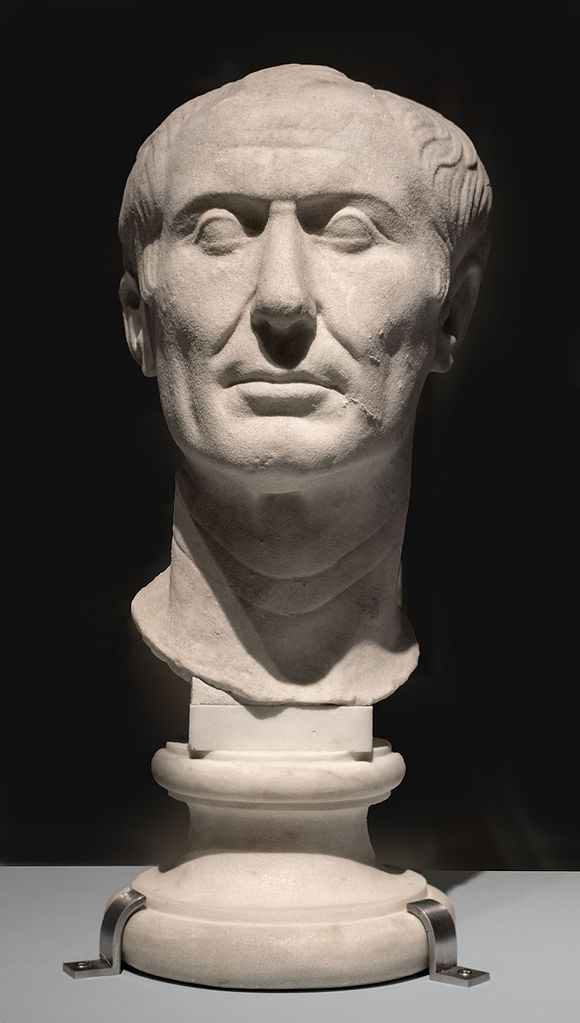
\includegraphics[width=0.5\textwidth]{figures/ceasar.jpg}\\
				\hspace*{15pt}\hbox{\scriptsize Image By:\thinspace{\itshape Ángel M. Felicísimo}}
				%https://commons.wikimedia.org/wiki/File:Retrato_de_Julio_C%C3%A9sar_(26724093101).jpg
			\end{center}

			\column{0.455\textwidth}
			\begin{center}
				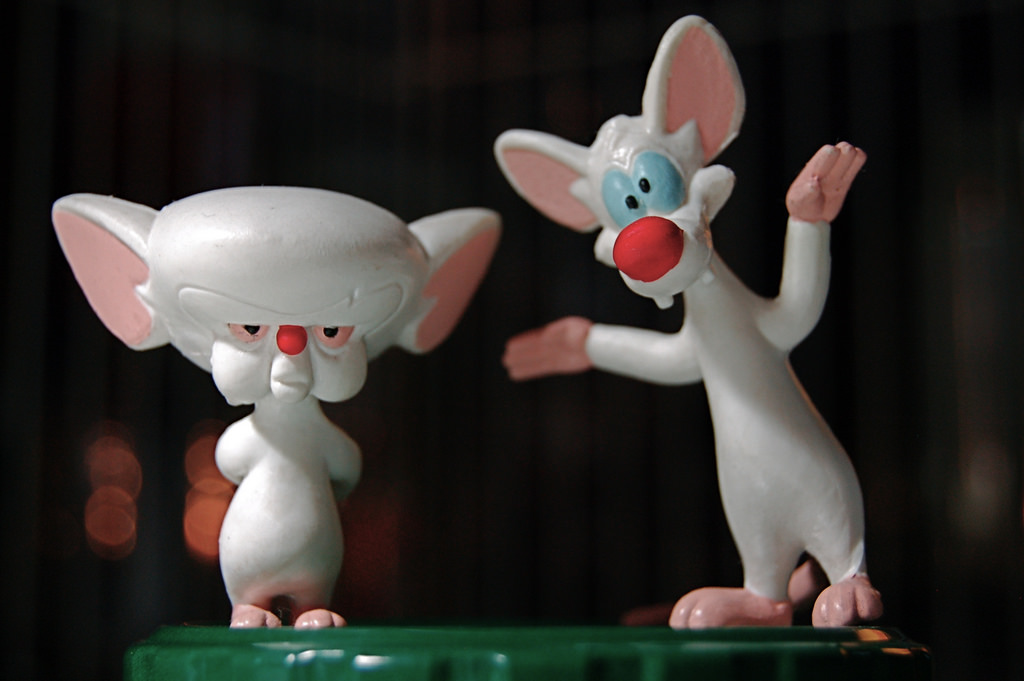
\includegraphics[width=0.9\textwidth]{figures/pinky.jpg}\\
				\hspace*{15pt}\hbox{\scriptsize Image By:\thinspace{\itshape JD Hancock}}
				%https://commons.wikimedia.org/wiki/File:Retrato_de_Julio_C%C3%A9sar_(26724093101).jpg

			\end{center}
		\end{columns}
\end{frame}

\begin{frame}
	\frametitle{Ideas for an algorithm}

	\begin{overlayarea}{\textwidth}{\textheight}
		\input{figures/tikz/closestpair_fixed.tex}
		
		\pause
		\begin{exampleblock}{Algorithm}
			\begin{itemize}
				\item \alert<2>{Divide}: Draw vertical line $L$ that has roughly half of the points on each side.
					\pause
				\item \alert<3>{Conquer}: Find the closest pair on each side.
					\pause
				\item \alert<4>{Combine}: Find the closest pair with one point on each side.
					\pause
				\item Return the minimum of these 3.
			\end{itemize}
		\end{exampleblock}	
	\end{overlayarea}
\end{frame}

\begin{frame}
	\frametitle{Did we make things better?}
	\begin{questionblock}{What is the run time of combine?}
		How much time to combine the two halves? Remember that we want to improve over $\Theta(n^2)$.
	\end{questionblock}	
\end{frame}

\begin{frame}
	\frametitle{How do we make it better?}
		\input{figures/tikz/closestpair_fixed2.tex}
	Observation:
	\begin{itemize}
		\item If $\delta$ is the minimum of the smallest distances left and right.
			\pause
		\item Then we only need to consider pairs of points within $\delta$ of $L$.
			\pause
		\item So in this example, none at all!
	\end{itemize}
\end{frame}

\begin{frame}
	\frametitle{Worst-case?}
	\begin{overlayarea}{\textwidth}{\textheight}
			\begin{itemize}
				\item But worst-case all points are in this $2\delta$-strip...
					\pause
				\item But if we sort them by $y$-coordinate (which can be done in $O(n\log n)$), then how many comparisons do we need?
					\pause
				\item Still $O(n^2)$!?
					\only<4->{
				\item Nope! We only need to check within 11 (i.e. a constant number of) positions in the sorted list.
				}
					\only<5->{
				\item So the combining step is $O(n \log n)$ (which can be further improved to $O(n)$)!
				}
			\end{itemize}
			\only<3>{
			\begin{center}
				
\includegraphics[width=0.4\textwidth]{figures/dilbert.jpg}
				\framesubtitle{http://thecontextofthings.com/wp-content/uploads/2017/11/dilbert-work.jpg}
			\end{center}
		}
	\end{overlayarea}
\end{frame}

\begin{frame}
	\frametitle{Why 11?}

	\begin{overlayarea}{\textwidth}{\textheight}
		\begin{columns}
			\column{0.655\textwidth}
			\begin{block}{Definition}
				Let $s_i$ be the point in the $2\delta$-strip with the $i^\text{th}$ smallest $y$-coordinate.
			\end{block}	
			
			\pause
			\begin{block}{Claim about 11}
				If $|i-j| > 11$ then the distance between $s_i$ and $s_j$ is at least $\delta$.
			\end{block}
			\column{0.255\textwidth}
			\input{figures/tikz/closestpair_delta.tex}	
		\end{columns}
		
		\pause
		\only<3-5>{
			\begin{block}{Proof sketch}
			\begin{itemize}
				\item No two points are in the same $0.5\delta$-by-$0.5\delta$-box.
					\only<4->{
				\item Two points that have two rows between them have a distance $\geq 2\cdot(0.5\delta) = \delta$.
				}
				\only<5->{
				\item So we only consider points at most 2 rows away.
				}
			\end{itemize}
		\end{block}
	}
	\only<6->{
		\begin{exampleblock}{Fun facts!}
			\begin{itemize}
				\item We can even reduce this to just 7 points.
					\only<7>{
				\item Even less if we consider columns separately.
				}
			\end{itemize}
		\end{exampleblock}	
	}
		
		\only<3>{
		\begin{questionblock}{Why not?}
			Why are there no two points in the same box?
		\end{questionblock}
}
	\end{overlayarea}
\end{frame}

\begin{frame}
	\frametitle{The algorithm}
	\begin{columns}
		\column{0.705\textwidth}
	\begin{algorithmic}
		\State Sort all points by x-coordinate
		\Function{Closest-Pair}{$p_1,\dots,p_n$}
			\If{n=1}
				\State \Return $\infty$
			\EndIf

			\pause
			\State $L \gets$ \alert<2>{median} $x$-coordinate
			\State $\delta_1 \gets$ \Call{Closest-Pair}{Points left of $L$}
			\State $\delta_2 \gets$ \Call{Closest-Pair}{Points right of $L$}
			\State $\delta \gets \min(\delta_1,\delta_2)$
			\pause
			\State get list of all points within $\delta$ from L.
			\State sort this list by y-coordinate
			\pause
			\State Scan by y-order, compare every point to the next 11 and update $\delta$ as you go.
			\State \Return $\delta$
		\EndFunction
	\end{algorithmic}
		\pnote{Why not the average?}
		\column{0.205\textwidth}
		\pause
		\begin{questionblock}{}
			What is the recurrence equation for the run time?	
		\end{questionblock}	
		\pause
		\begin{answerblock}{}
			\small
			$T(n) =2T(n/2) + O(n\log n)$	
		\end{answerblock}
	\end{columns}
	
\end{frame}

	\pnote{Why is this relevant? Answers: For instance collision detection algorithms}
\end{frame}

\begin{frame}
	\frametitle{Let's just brute-force it?}
	\begin{overlayarea}{\textwidth}{\textheight}
		\section{Closest pair of points}
\label{sec:closest_pair_of_points}


\begin{frame}
	\frametitle{A new problem}
	\begin{problemblock}{Closest pair of points}
		Given a set of points, what is the pair of points that is closest to each other?\\
		\pause
		More formally:
		\begin{itemize}
			\item Given a set of points $S$, where every point $p_i$ has an x-coordinate $x_i$ and y-coordinate $y_i$.
			\item Distance is defined as: $d(i,j) = \sqrt{{(x_i - x_j)}^{2} + {(y_i-y_j)}^2}$
			\item What is the pair of points $i,j$ such that $d(i,j)$ is minimal?
		\end{itemize}
	\end{problemblock}
	\pause
	\input{figures/tikz/closestpair.tex}
	\pnote{Why is this relevant? Answers: For instance collision detection algorithms}
\end{frame}

\begin{frame}
	\frametitle{Let's just brute-force it?}
	\begin{overlayarea}{\textwidth}{\textheight}
		\input{figures/tikz/closestpair.tex}
		\begin{questionblock}{Brute-force}
			What is the tightest upper bound on the run time for a brute-force solution given $|S| = n$?
			\only<2>{
			\begin{enumerate}[A.]
				\item $O(n \log n)$
				\item $O(n^2)$
				\item $O(n^2 \log n)$
				\item $O(n^3)$
				\item I don't know.
			\end{enumerate}
		}
		\end{questionblock}
		\only<3>{
			\begin{answerblock}{Try every combination}
				We check every pair of points, of which there are $n^2$, so $O(n^2)$.	
			\end{answerblock}
		}
	\end{overlayarea}
\end{frame}

\begin{frame}
	\frametitle{Time to improve!}
	\framesubtitle{Using Divide \& Conquer}
		\begin{columns}
			\column{0.455\textwidth}
			\begin{center}
				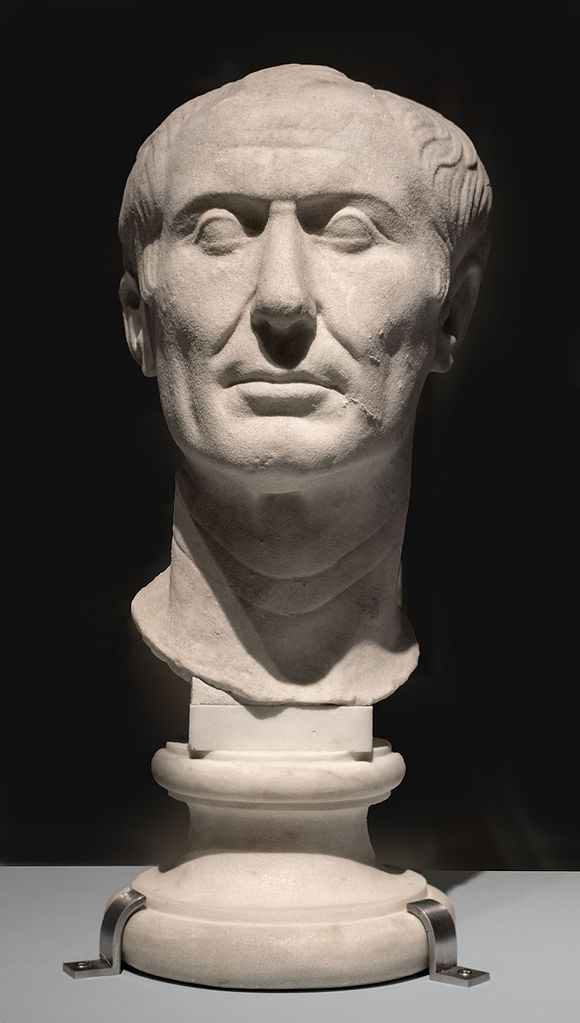
\includegraphics[width=0.5\textwidth]{figures/ceasar.jpg}\\
				\hspace*{15pt}\hbox{\scriptsize Image By:\thinspace{\itshape Ángel M. Felicísimo}}
				%https://commons.wikimedia.org/wiki/File:Retrato_de_Julio_C%C3%A9sar_(26724093101).jpg
			\end{center}

			\column{0.455\textwidth}
			\begin{center}
				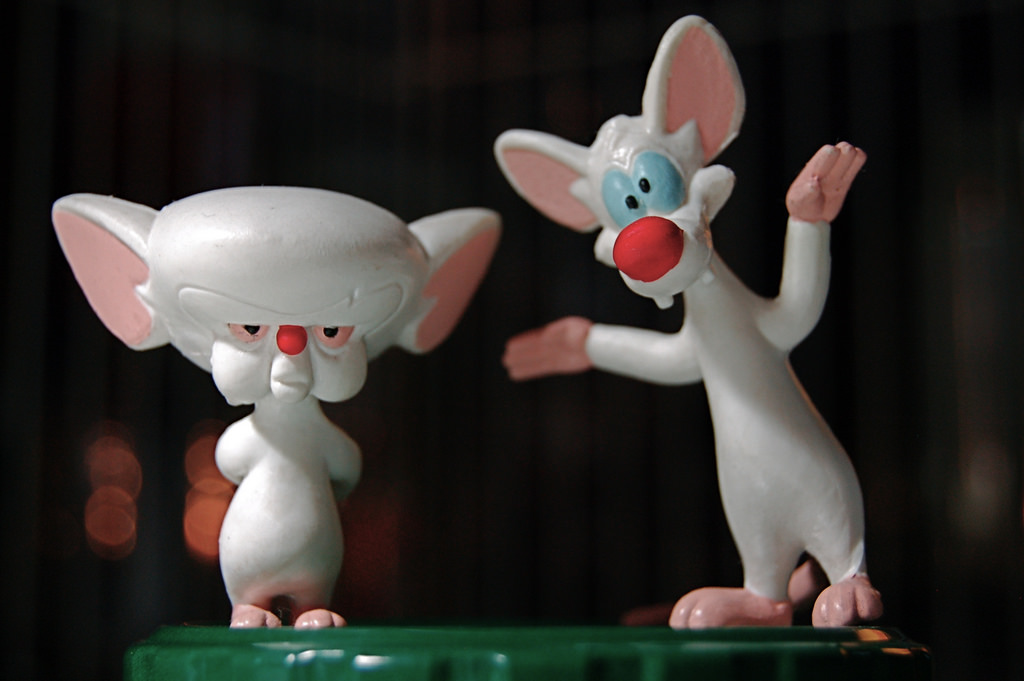
\includegraphics[width=0.9\textwidth]{figures/pinky.jpg}\\
				\hspace*{15pt}\hbox{\scriptsize Image By:\thinspace{\itshape JD Hancock}}
				%https://commons.wikimedia.org/wiki/File:Retrato_de_Julio_C%C3%A9sar_(26724093101).jpg

			\end{center}
		\end{columns}
\end{frame}

\begin{frame}
	\frametitle{Ideas for an algorithm}

	\begin{overlayarea}{\textwidth}{\textheight}
		\input{figures/tikz/closestpair_fixed.tex}
		
		\pause
		\begin{exampleblock}{Algorithm}
			\begin{itemize}
				\item \alert<2>{Divide}: Draw vertical line $L$ that has roughly half of the points on each side.
					\pause
				\item \alert<3>{Conquer}: Find the closest pair on each side.
					\pause
				\item \alert<4>{Combine}: Find the closest pair with one point on each side.
					\pause
				\item Return the minimum of these 3.
			\end{itemize}
		\end{exampleblock}	
	\end{overlayarea}
\end{frame}

\begin{frame}
	\frametitle{Did we make things better?}
	\begin{questionblock}{What is the run time of combine?}
		How much time to combine the two halves? Remember that we want to improve over $\Theta(n^2)$.
	\end{questionblock}	
\end{frame}

\begin{frame}
	\frametitle{How do we make it better?}
		\input{figures/tikz/closestpair_fixed2.tex}
	Observation:
	\begin{itemize}
		\item If $\delta$ is the minimum of the smallest distances left and right.
			\pause
		\item Then we only need to consider pairs of points within $\delta$ of $L$.
			\pause
		\item So in this example, none at all!
	\end{itemize}
\end{frame}

\begin{frame}
	\frametitle{Worst-case?}
	\begin{overlayarea}{\textwidth}{\textheight}
			\begin{itemize}
				\item But worst-case all points are in this $2\delta$-strip...
					\pause
				\item But if we sort them by $y$-coordinate (which can be done in $O(n\log n)$), then how many comparisons do we need?
					\pause
				\item Still $O(n^2)$!?
					\only<4->{
				\item Nope! We only need to check within 11 (i.e. a constant number of) positions in the sorted list.
				}
					\only<5->{
				\item So the combining step is $O(n \log n)$ (which can be further improved to $O(n)$)!
				}
			\end{itemize}
			\only<3>{
			\begin{center}
				
\includegraphics[width=0.4\textwidth]{figures/dilbert.jpg}
				\framesubtitle{http://thecontextofthings.com/wp-content/uploads/2017/11/dilbert-work.jpg}
			\end{center}
		}
	\end{overlayarea}
\end{frame}

\begin{frame}
	\frametitle{Why 11?}

	\begin{overlayarea}{\textwidth}{\textheight}
		\begin{columns}
			\column{0.655\textwidth}
			\begin{block}{Definition}
				Let $s_i$ be the point in the $2\delta$-strip with the $i^\text{th}$ smallest $y$-coordinate.
			\end{block}	
			
			\pause
			\begin{block}{Claim about 11}
				If $|i-j| > 11$ then the distance between $s_i$ and $s_j$ is at least $\delta$.
			\end{block}
			\column{0.255\textwidth}
			\input{figures/tikz/closestpair_delta.tex}	
		\end{columns}
		
		\pause
		\only<3-5>{
			\begin{block}{Proof sketch}
			\begin{itemize}
				\item No two points are in the same $0.5\delta$-by-$0.5\delta$-box.
					\only<4->{
				\item Two points that have two rows between them have a distance $\geq 2\cdot(0.5\delta) = \delta$.
				}
				\only<5->{
				\item So we only consider points at most 2 rows away.
				}
			\end{itemize}
		\end{block}
	}
	\only<6->{
		\begin{exampleblock}{Fun facts!}
			\begin{itemize}
				\item We can even reduce this to just 7 points.
					\only<7>{
				\item Even less if we consider columns separately.
				}
			\end{itemize}
		\end{exampleblock}	
	}
		
		\only<3>{
		\begin{questionblock}{Why not?}
			Why are there no two points in the same box?
		\end{questionblock}
}
	\end{overlayarea}
\end{frame}

\begin{frame}
	\frametitle{The algorithm}
	\begin{columns}
		\column{0.705\textwidth}
	\begin{algorithmic}
		\State Sort all points by x-coordinate
		\Function{Closest-Pair}{$p_1,\dots,p_n$}
			\If{n=1}
				\State \Return $\infty$
			\EndIf

			\pause
			\State $L \gets$ \alert<2>{median} $x$-coordinate
			\State $\delta_1 \gets$ \Call{Closest-Pair}{Points left of $L$}
			\State $\delta_2 \gets$ \Call{Closest-Pair}{Points right of $L$}
			\State $\delta \gets \min(\delta_1,\delta_2)$
			\pause
			\State get list of all points within $\delta$ from L.
			\State sort this list by y-coordinate
			\pause
			\State Scan by y-order, compare every point to the next 11 and update $\delta$ as you go.
			\State \Return $\delta$
		\EndFunction
	\end{algorithmic}
		\pnote{Why not the average?}
		\column{0.205\textwidth}
		\pause
		\begin{questionblock}{}
			What is the recurrence equation for the run time?	
		\end{questionblock}	
		\pause
		\begin{answerblock}{}
			\small
			$T(n) =2T(n/2) + O(n\log n)$	
		\end{answerblock}
	\end{columns}
	
\end{frame}

		\begin{questionblock}{Brute-force}
			What is the tightest upper bound on the run time for a brute-force solution given $|S| = n$?
			\only<2>{
			\begin{enumerate}[A.]
				\item $O(n \log n)$
				\item $O(n^2)$
				\item $O(n^2 \log n)$
				\item $O(n^3)$
				\item I don't know.
			\end{enumerate}
		}
		\end{questionblock}
		\only<3>{
			\begin{answerblock}{Try every combination}
				We check every pair of points, of which there are $n^2$, so $O(n^2)$.	
			\end{answerblock}
		}
	\end{overlayarea}
\end{frame}

\begin{frame}
	\frametitle{Time to improve!}
	\framesubtitle{Using Divide \& Conquer}
		\begin{columns}
			\column{0.455\textwidth}
			\begin{center}
				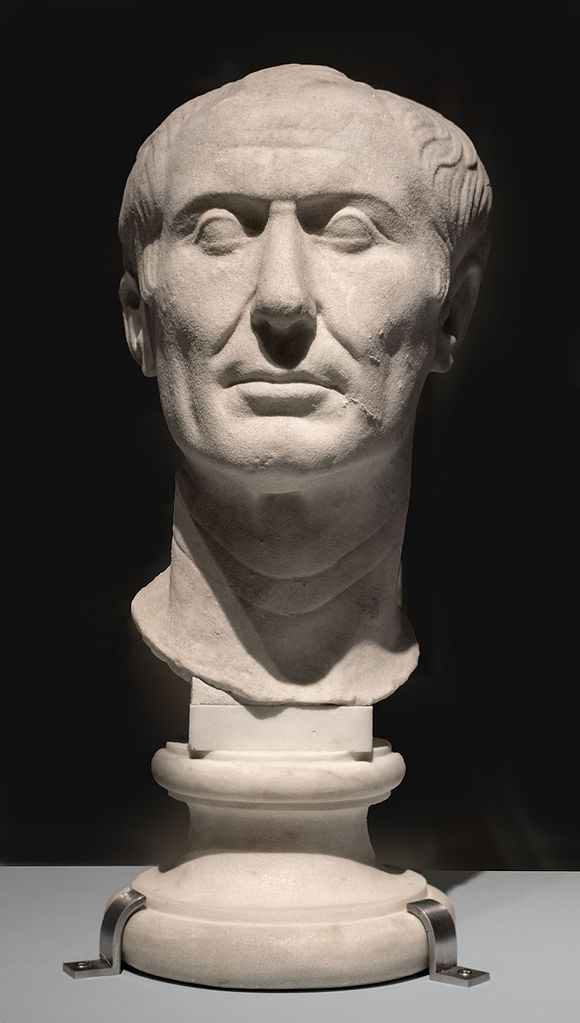
\includegraphics[width=0.5\textwidth]{figures/ceasar.jpg}\\
				\hspace*{15pt}\hbox{\scriptsize Image By:\thinspace{\itshape Ángel M. Felicísimo}}
				%https://commons.wikimedia.org/wiki/File:Retrato_de_Julio_C%C3%A9sar_(26724093101).jpg
			\end{center}

			\column{0.455\textwidth}
			\begin{center}
				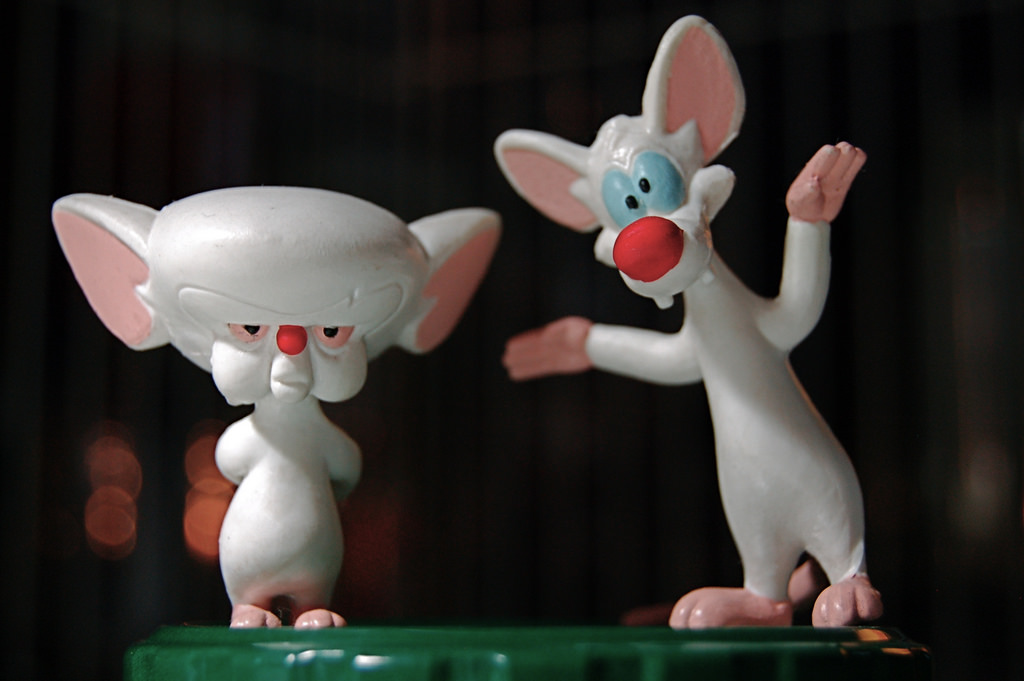
\includegraphics[width=0.9\textwidth]{figures/pinky.jpg}\\
				\hspace*{15pt}\hbox{\scriptsize Image By:\thinspace{\itshape JD Hancock}}
				%https://commons.wikimedia.org/wiki/File:Retrato_de_Julio_C%C3%A9sar_(26724093101).jpg

			\end{center}
		\end{columns}
\end{frame}

\begin{frame}
	\frametitle{Ideas for an algorithm}

	\begin{overlayarea}{\textwidth}{\textheight}
		\begin{figure}[htpb]
\begin{center}
\begin{tikzpicture}[scale=0.5, transform shape]
	\draw (-8,-3) rectangle (8,3);

	\foreach \x/\y/\name in {
		-7/2/,
		-6/1/l1,
		-5/1/l2,
		-3/-2/c1,
		-1/-2/c2,
		3/-1/,
		5/1.5/r1,
		5/0/r2,
		}{
		\node[circle, black, draw, fill=blue!30, minimum size=4pt] (\name) at (\x,\y) {};
	}
		\node at (-1.5, -3.5) {};
	\only<2->{
		\draw[dotted] (-1.5,-3) -- (-1.5,3);
		\node at (-1.5, -3.5) {\Large $L$};
	}
	\only<3->{
		\draw[dotted, red, thick] (l1) --  node[anchor=south] {\Large 1} (l2);
		\draw[dotted, red, thick] (r1) --  node[anchor=west] {\Large 1.5} (r2);
	}
	\only<4->{
		\draw[dotted, red, thick] (c1) --  node[anchor=south] {\Large 2} (c2);
	}
\end{tikzpicture}
\end{center}
\end{figure}

		
		\pause
		\begin{exampleblock}{Algorithm}
			\begin{itemize}
				\item \alert<2>{Divide}: Draw vertical line $L$ that has roughly half of the points on each side.
					\pause
				\item \alert<3>{Conquer}: Find the closest pair on each side.
					\pause
				\item \alert<4>{Combine}: Find the closest pair with one point on each side.
					\pause
				\item Return the minimum of these 3.
			\end{itemize}
		\end{exampleblock}	
	\end{overlayarea}
\end{frame}

\begin{frame}
	\frametitle{Did we make things better?}
	\begin{questionblock}{What is the run time of combine?}
		How much time to combine the two halves? Remember that we want to improve over $\Theta(n^2)$.
	\end{questionblock}	
\end{frame}

\begin{frame}
	\frametitle{How do we make it better?}
		\begin{figure}[htpb]
\begin{center}
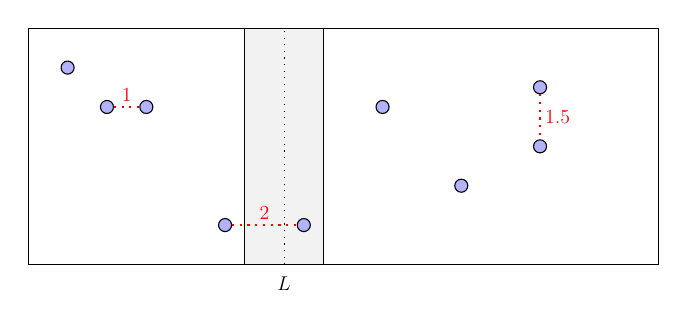
\begin{tikzpicture}[scale=0.5, transform shape]
	\draw (-8,-3) rectangle (8,3);

	\only<2->{
		\draw[fill=gray!10] (-2.5,-3) rectangle (-0.5,3);
	}
	\foreach \x/\y/\name in {
		-7/2/,
		-6/1/l1,
		-5/1/l2,
		-3/-2/c1,
		-1/-2/c2,
		3/-1/,
		5/1.5/r1,
		5/0/r2,
		}{
		\node[circle, black, draw, fill=blue!30, minimum size=4pt] (\name) at (\x,\y) {};
	}
		\draw[dotted] (-1.5,-3) -- (-1.5,3);
		\node at (-1.5, -3.5) {\Large $L$};
		\draw[dotted, red, thick] (l1) --  node[anchor=south] {\Large 1} (l2);
		\draw[dotted, red, thick] (r1) --  node[anchor=west] {\Large 1.5} (r2);
		\draw[dotted, red, thick] (c1) --  node[anchor=south] {\Large 2} (c2);

\end{tikzpicture}
\end{center}
\end{figure}

	Observation:
	\begin{itemize}
		\item If $\delta$ is the minimum of the smallest distances left and right.
			\pause
		\item Then we only need to consider pairs of points within $\delta$ of $L$.
			\pause
		\item So in this example, none at all!
	\end{itemize}
\end{frame}

\begin{frame}
	\frametitle{Worst-case?}
	\begin{overlayarea}{\textwidth}{\textheight}
			\begin{itemize}
				\item But worst-case all points are in this $2\delta$-strip...
					\pause
				\item But if we sort them by $y$-coordinate (which can be done in $O(n\log n)$), then how many comparisons do we need?
					\pause
				\item Still $O(n^2)$!?
					\only<4->{
				\item Nope! We only need to check within 11 (i.e. a constant number of) positions in the sorted list.
				}
					\only<5->{
				\item So the combining step is $O(n \log n)$ (which can be further improved to $O(n)$)!
				}
			\end{itemize}
			\only<3>{
			\begin{center}
				
\includegraphics[width=0.4\textwidth]{figures/dilbert.jpg}
				\framesubtitle{http://thecontextofthings.com/wp-content/uploads/2017/11/dilbert-work.jpg}
			\end{center}
		}
	\end{overlayarea}
\end{frame}

\begin{frame}
	\frametitle{Why 11?}

	\begin{overlayarea}{\textwidth}{\textheight}
		\begin{columns}
			\column{0.655\textwidth}
			\begin{block}{Definition}
				Let $s_i$ be the point in the $2\delta$-strip with the $i^\text{th}$ smallest $y$-coordinate.
			\end{block}	
			
			\pause
			\begin{block}{Claim about 11}
				If $|i-j| > 11$ then the distance between $s_i$ and $s_j$ is at least $\delta$.
			\end{block}
			\column{0.255\textwidth}
			\begin{figure}[htpb]
\begin{center}
\begin{tikzpicture}[scale=0.4, transform shape]
	\draw (-2,-4) rectangle (2,4);
	
	\only<5->{
		\foreach \y in {-2, ..., 0}{
			\foreach \x in {-2, ..., 1}{
				\draw[fill=green!30] (\x,\y) rectangle (\x+1,\y+1);
			}
		}
	}

	\foreach \x/\y/\name/\color in {
		1.35/-2.4/1/red,
		-1.35/-1.6/2/green,
		-0.4/-0.4/3/blue,
		1.3/0.5/4/blue,
	%	1.7/1.4/5/red,
		-0.4/2.4/5/red,
		0.3/2.4/6/red}{
		\alt<4->{
		\node[circle, black, draw, fill=\color!30, minimum size=4pt] () at (\x,\y) {\name};
			}{
		\node[circle, black, draw, fill=blue!30, minimum size=4pt] () at (\x,\y) {\name};
		}
	}
		\draw[thick] (0,-4) -- (0,4);
		\node at (0, -4.5) {\Large $L$};
		\node at (-2, -4.5) {\Large $L-\delta$};
		\node at (2, -4.5) {\Large $L+\delta$};
		\only<3->{
			\draw[dotted] (1,-4) -- (1,4);
			\draw[dotted] (-1,-4) -- (-1,4);

			\foreach \y in {-3, ..., 3}{
				\draw[dotted] (-2,\y) -- (2,\y);
			}
		}

\end{tikzpicture}
\end{center}
\end{figure}
	
		\end{columns}
		
		\pause
		\only<3-5>{
			\begin{block}{Proof sketch}
			\begin{itemize}
				\item No two points are in the same $0.5\delta$-by-$0.5\delta$-box.
					\only<4->{
				\item Two points that have two rows between them have a distance $\geq 2\cdot(0.5\delta) = \delta$.
				}
				\only<5->{
				\item So we only consider points at most 2 rows away.
				}
			\end{itemize}
		\end{block}
	}
	\only<6->{
		\begin{exampleblock}{Fun facts!}
			\begin{itemize}
				\item We can even reduce this to just 7 points.
					\only<7>{
				\item Even less if we consider columns separately.
				}
			\end{itemize}
		\end{exampleblock}	
	}
		
		\only<3>{
		\begin{questionblock}{Why not?}
			Why are there no two points in the same box?
		\end{questionblock}
}
	\end{overlayarea}
\end{frame}

\begin{frame}
	\frametitle{The algorithm}
	\begin{columns}
		\column{0.705\textwidth}
	\begin{algorithmic}
		\State Sort all points by x-coordinate
		\Function{Closest-Pair}{$p_1,\dots,p_n$}
			\If{n=1}
				\State \Return $\infty$
			\EndIf

			\pause
			\State $L \gets$ \alert<2>{median} $x$-coordinate
			\State $\delta_1 \gets$ \Call{Closest-Pair}{Points left of $L$}
			\State $\delta_2 \gets$ \Call{Closest-Pair}{Points right of $L$}
			\State $\delta \gets \min(\delta_1,\delta_2)$
			\pause
			\State get list of all points within $\delta$ from L.
			\State sort this list by y-coordinate
			\pause
			\State Scan by y-order, compare every point to the next 11 and update $\delta$ as you go.
			\State \Return $\delta$
		\EndFunction
	\end{algorithmic}
		\pnote{Why not the average?}
		\column{0.205\textwidth}
		\pause
		\begin{questionblock}{}
			What is the recurrence equation for the run time?	
		\end{questionblock}	
		\pause
		\begin{answerblock}{}
			\small
			$T(n) =2T(n/2) + O(n\log n)$	
		\end{answerblock}
	\end{columns}
	
\end{frame}

	\pnote{Why is this relevant? Answers: For instance collision detection algorithms}
\end{frame}

\begin{frame}
	\frametitle{Let's just brute-force it?}
	\begin{overlayarea}{\textwidth}{\textheight}
		\section{Closest pair of points}
\label{sec:closest_pair_of_points}


\begin{frame}
	\frametitle{A new problem}
	\begin{problemblock}{Closest pair of points}
		Given a set of points, what is the pair of points that is closest to each other?\\
		\pause
		More formally:
		\begin{itemize}
			\item Given a set of points $S$, where every point $p_i$ has an x-coordinate $x_i$ and y-coordinate $y_i$.
			\item Distance is defined as: $d(i,j) = \sqrt{{(x_i - x_j)}^{2} + {(y_i-y_j)}^2}$
			\item What is the pair of points $i,j$ such that $d(i,j)$ is minimal?
		\end{itemize}
	\end{problemblock}
	\pause
	\section{Closest pair of points}
\label{sec:closest_pair_of_points}


\begin{frame}
	\frametitle{A new problem}
	\begin{problemblock}{Closest pair of points}
		Given a set of points, what is the pair of points that is closest to each other?\\
		\pause
		More formally:
		\begin{itemize}
			\item Given a set of points $S$, where every point $p_i$ has an x-coordinate $x_i$ and y-coordinate $y_i$.
			\item Distance is defined as: $d(i,j) = \sqrt{{(x_i - x_j)}^{2} + {(y_i-y_j)}^2}$
			\item What is the pair of points $i,j$ such that $d(i,j)$ is minimal?
		\end{itemize}
	\end{problemblock}
	\pause
	\input{figures/tikz/closestpair.tex}
	\pnote{Why is this relevant? Answers: For instance collision detection algorithms}
\end{frame}

\begin{frame}
	\frametitle{Let's just brute-force it?}
	\begin{overlayarea}{\textwidth}{\textheight}
		\input{figures/tikz/closestpair.tex}
		\begin{questionblock}{Brute-force}
			What is the tightest upper bound on the run time for a brute-force solution given $|S| = n$?
			\only<2>{
			\begin{enumerate}[A.]
				\item $O(n \log n)$
				\item $O(n^2)$
				\item $O(n^2 \log n)$
				\item $O(n^3)$
				\item I don't know.
			\end{enumerate}
		}
		\end{questionblock}
		\only<3>{
			\begin{answerblock}{Try every combination}
				We check every pair of points, of which there are $n^2$, so $O(n^2)$.	
			\end{answerblock}
		}
	\end{overlayarea}
\end{frame}

\begin{frame}
	\frametitle{Time to improve!}
	\framesubtitle{Using Divide \& Conquer}
		\begin{columns}
			\column{0.455\textwidth}
			\begin{center}
				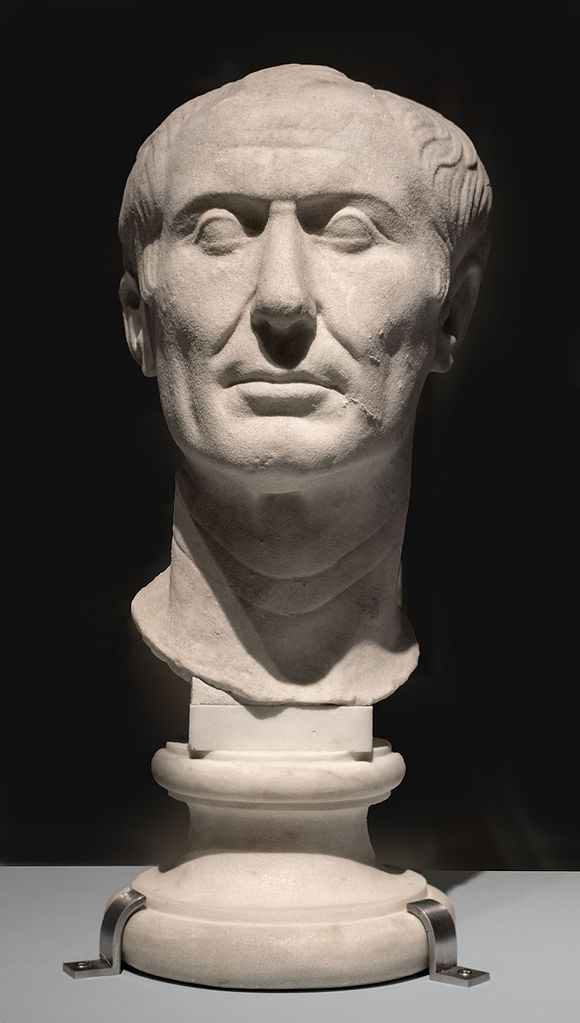
\includegraphics[width=0.5\textwidth]{figures/ceasar.jpg}\\
				\hspace*{15pt}\hbox{\scriptsize Image By:\thinspace{\itshape Ángel M. Felicísimo}}
				%https://commons.wikimedia.org/wiki/File:Retrato_de_Julio_C%C3%A9sar_(26724093101).jpg
			\end{center}

			\column{0.455\textwidth}
			\begin{center}
				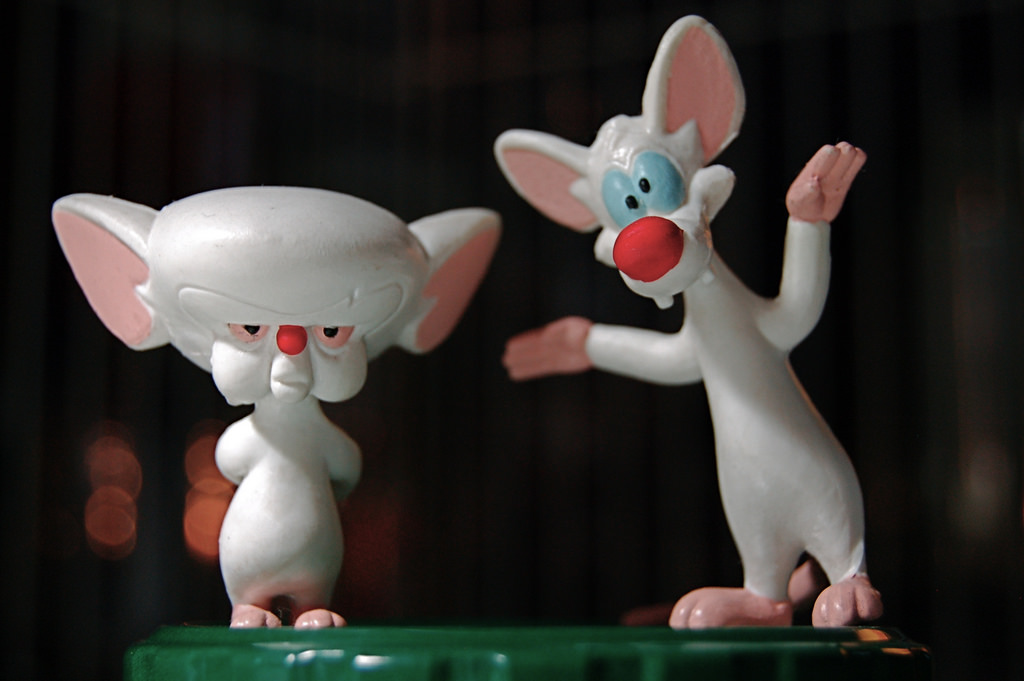
\includegraphics[width=0.9\textwidth]{figures/pinky.jpg}\\
				\hspace*{15pt}\hbox{\scriptsize Image By:\thinspace{\itshape JD Hancock}}
				%https://commons.wikimedia.org/wiki/File:Retrato_de_Julio_C%C3%A9sar_(26724093101).jpg

			\end{center}
		\end{columns}
\end{frame}

\begin{frame}
	\frametitle{Ideas for an algorithm}

	\begin{overlayarea}{\textwidth}{\textheight}
		\input{figures/tikz/closestpair_fixed.tex}
		
		\pause
		\begin{exampleblock}{Algorithm}
			\begin{itemize}
				\item \alert<2>{Divide}: Draw vertical line $L$ that has roughly half of the points on each side.
					\pause
				\item \alert<3>{Conquer}: Find the closest pair on each side.
					\pause
				\item \alert<4>{Combine}: Find the closest pair with one point on each side.
					\pause
				\item Return the minimum of these 3.
			\end{itemize}
		\end{exampleblock}	
	\end{overlayarea}
\end{frame}

\begin{frame}
	\frametitle{Did we make things better?}
	\begin{questionblock}{What is the run time of combine?}
		How much time to combine the two halves? Remember that we want to improve over $\Theta(n^2)$.
	\end{questionblock}	
\end{frame}

\begin{frame}
	\frametitle{How do we make it better?}
		\input{figures/tikz/closestpair_fixed2.tex}
	Observation:
	\begin{itemize}
		\item If $\delta$ is the minimum of the smallest distances left and right.
			\pause
		\item Then we only need to consider pairs of points within $\delta$ of $L$.
			\pause
		\item So in this example, none at all!
	\end{itemize}
\end{frame}

\begin{frame}
	\frametitle{Worst-case?}
	\begin{overlayarea}{\textwidth}{\textheight}
			\begin{itemize}
				\item But worst-case all points are in this $2\delta$-strip...
					\pause
				\item But if we sort them by $y$-coordinate (which can be done in $O(n\log n)$), then how many comparisons do we need?
					\pause
				\item Still $O(n^2)$!?
					\only<4->{
				\item Nope! We only need to check within 11 (i.e. a constant number of) positions in the sorted list.
				}
					\only<5->{
				\item So the combining step is $O(n \log n)$ (which can be further improved to $O(n)$)!
				}
			\end{itemize}
			\only<3>{
			\begin{center}
				
\includegraphics[width=0.4\textwidth]{figures/dilbert.jpg}
				\framesubtitle{http://thecontextofthings.com/wp-content/uploads/2017/11/dilbert-work.jpg}
			\end{center}
		}
	\end{overlayarea}
\end{frame}

\begin{frame}
	\frametitle{Why 11?}

	\begin{overlayarea}{\textwidth}{\textheight}
		\begin{columns}
			\column{0.655\textwidth}
			\begin{block}{Definition}
				Let $s_i$ be the point in the $2\delta$-strip with the $i^\text{th}$ smallest $y$-coordinate.
			\end{block}	
			
			\pause
			\begin{block}{Claim about 11}
				If $|i-j| > 11$ then the distance between $s_i$ and $s_j$ is at least $\delta$.
			\end{block}
			\column{0.255\textwidth}
			\input{figures/tikz/closestpair_delta.tex}	
		\end{columns}
		
		\pause
		\only<3-5>{
			\begin{block}{Proof sketch}
			\begin{itemize}
				\item No two points are in the same $0.5\delta$-by-$0.5\delta$-box.
					\only<4->{
				\item Two points that have two rows between them have a distance $\geq 2\cdot(0.5\delta) = \delta$.
				}
				\only<5->{
				\item So we only consider points at most 2 rows away.
				}
			\end{itemize}
		\end{block}
	}
	\only<6->{
		\begin{exampleblock}{Fun facts!}
			\begin{itemize}
				\item We can even reduce this to just 7 points.
					\only<7>{
				\item Even less if we consider columns separately.
				}
			\end{itemize}
		\end{exampleblock}	
	}
		
		\only<3>{
		\begin{questionblock}{Why not?}
			Why are there no two points in the same box?
		\end{questionblock}
}
	\end{overlayarea}
\end{frame}

\begin{frame}
	\frametitle{The algorithm}
	\begin{columns}
		\column{0.705\textwidth}
	\begin{algorithmic}
		\State Sort all points by x-coordinate
		\Function{Closest-Pair}{$p_1,\dots,p_n$}
			\If{n=1}
				\State \Return $\infty$
			\EndIf

			\pause
			\State $L \gets$ \alert<2>{median} $x$-coordinate
			\State $\delta_1 \gets$ \Call{Closest-Pair}{Points left of $L$}
			\State $\delta_2 \gets$ \Call{Closest-Pair}{Points right of $L$}
			\State $\delta \gets \min(\delta_1,\delta_2)$
			\pause
			\State get list of all points within $\delta$ from L.
			\State sort this list by y-coordinate
			\pause
			\State Scan by y-order, compare every point to the next 11 and update $\delta$ as you go.
			\State \Return $\delta$
		\EndFunction
	\end{algorithmic}
		\pnote{Why not the average?}
		\column{0.205\textwidth}
		\pause
		\begin{questionblock}{}
			What is the recurrence equation for the run time?	
		\end{questionblock}	
		\pause
		\begin{answerblock}{}
			\small
			$T(n) =2T(n/2) + O(n\log n)$	
		\end{answerblock}
	\end{columns}
	
\end{frame}

	\pnote{Why is this relevant? Answers: For instance collision detection algorithms}
\end{frame}

\begin{frame}
	\frametitle{Let's just brute-force it?}
	\begin{overlayarea}{\textwidth}{\textheight}
		\section{Closest pair of points}
\label{sec:closest_pair_of_points}


\begin{frame}
	\frametitle{A new problem}
	\begin{problemblock}{Closest pair of points}
		Given a set of points, what is the pair of points that is closest to each other?\\
		\pause
		More formally:
		\begin{itemize}
			\item Given a set of points $S$, where every point $p_i$ has an x-coordinate $x_i$ and y-coordinate $y_i$.
			\item Distance is defined as: $d(i,j) = \sqrt{{(x_i - x_j)}^{2} + {(y_i-y_j)}^2}$
			\item What is the pair of points $i,j$ such that $d(i,j)$ is minimal?
		\end{itemize}
	\end{problemblock}
	\pause
	\input{figures/tikz/closestpair.tex}
	\pnote{Why is this relevant? Answers: For instance collision detection algorithms}
\end{frame}

\begin{frame}
	\frametitle{Let's just brute-force it?}
	\begin{overlayarea}{\textwidth}{\textheight}
		\input{figures/tikz/closestpair.tex}
		\begin{questionblock}{Brute-force}
			What is the tightest upper bound on the run time for a brute-force solution given $|S| = n$?
			\only<2>{
			\begin{enumerate}[A.]
				\item $O(n \log n)$
				\item $O(n^2)$
				\item $O(n^2 \log n)$
				\item $O(n^3)$
				\item I don't know.
			\end{enumerate}
		}
		\end{questionblock}
		\only<3>{
			\begin{answerblock}{Try every combination}
				We check every pair of points, of which there are $n^2$, so $O(n^2)$.	
			\end{answerblock}
		}
	\end{overlayarea}
\end{frame}

\begin{frame}
	\frametitle{Time to improve!}
	\framesubtitle{Using Divide \& Conquer}
		\begin{columns}
			\column{0.455\textwidth}
			\begin{center}
				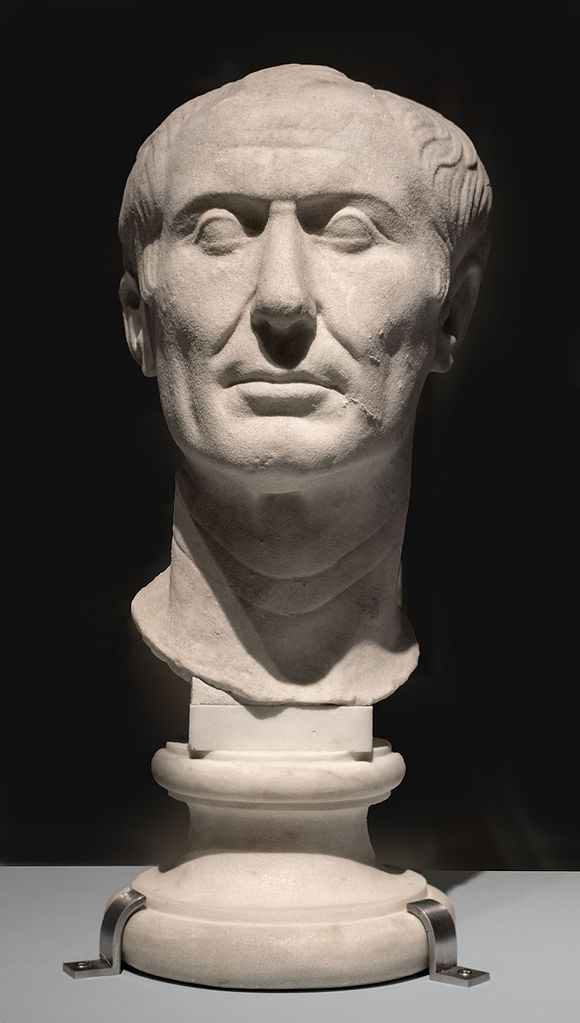
\includegraphics[width=0.5\textwidth]{figures/ceasar.jpg}\\
				\hspace*{15pt}\hbox{\scriptsize Image By:\thinspace{\itshape Ángel M. Felicísimo}}
				%https://commons.wikimedia.org/wiki/File:Retrato_de_Julio_C%C3%A9sar_(26724093101).jpg
			\end{center}

			\column{0.455\textwidth}
			\begin{center}
				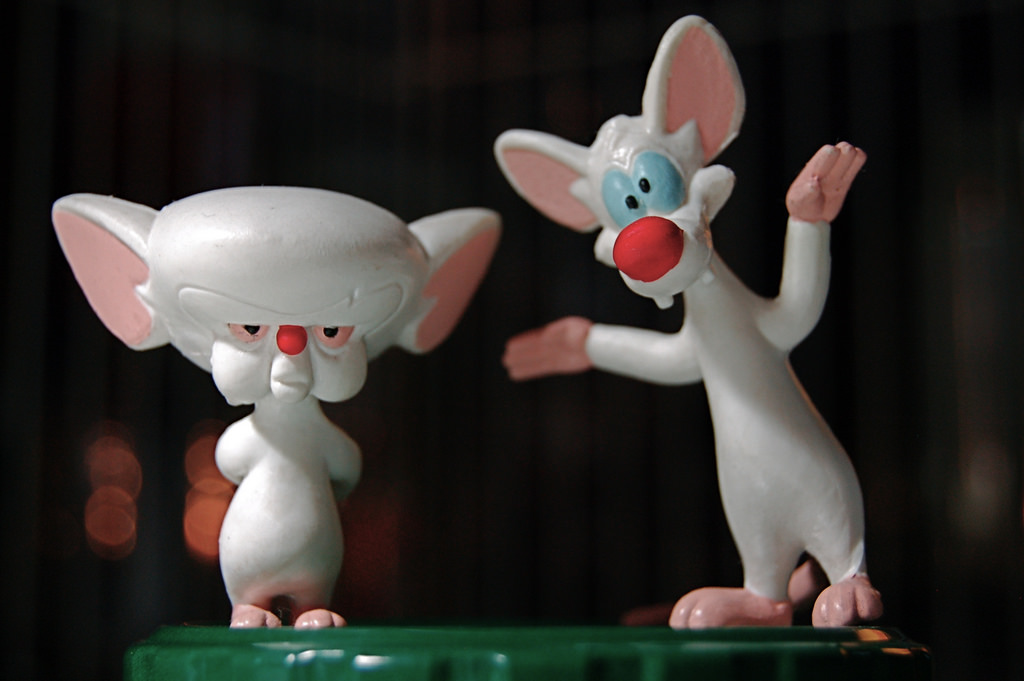
\includegraphics[width=0.9\textwidth]{figures/pinky.jpg}\\
				\hspace*{15pt}\hbox{\scriptsize Image By:\thinspace{\itshape JD Hancock}}
				%https://commons.wikimedia.org/wiki/File:Retrato_de_Julio_C%C3%A9sar_(26724093101).jpg

			\end{center}
		\end{columns}
\end{frame}

\begin{frame}
	\frametitle{Ideas for an algorithm}

	\begin{overlayarea}{\textwidth}{\textheight}
		\input{figures/tikz/closestpair_fixed.tex}
		
		\pause
		\begin{exampleblock}{Algorithm}
			\begin{itemize}
				\item \alert<2>{Divide}: Draw vertical line $L$ that has roughly half of the points on each side.
					\pause
				\item \alert<3>{Conquer}: Find the closest pair on each side.
					\pause
				\item \alert<4>{Combine}: Find the closest pair with one point on each side.
					\pause
				\item Return the minimum of these 3.
			\end{itemize}
		\end{exampleblock}	
	\end{overlayarea}
\end{frame}

\begin{frame}
	\frametitle{Did we make things better?}
	\begin{questionblock}{What is the run time of combine?}
		How much time to combine the two halves? Remember that we want to improve over $\Theta(n^2)$.
	\end{questionblock}	
\end{frame}

\begin{frame}
	\frametitle{How do we make it better?}
		\input{figures/tikz/closestpair_fixed2.tex}
	Observation:
	\begin{itemize}
		\item If $\delta$ is the minimum of the smallest distances left and right.
			\pause
		\item Then we only need to consider pairs of points within $\delta$ of $L$.
			\pause
		\item So in this example, none at all!
	\end{itemize}
\end{frame}

\begin{frame}
	\frametitle{Worst-case?}
	\begin{overlayarea}{\textwidth}{\textheight}
			\begin{itemize}
				\item But worst-case all points are in this $2\delta$-strip...
					\pause
				\item But if we sort them by $y$-coordinate (which can be done in $O(n\log n)$), then how many comparisons do we need?
					\pause
				\item Still $O(n^2)$!?
					\only<4->{
				\item Nope! We only need to check within 11 (i.e. a constant number of) positions in the sorted list.
				}
					\only<5->{
				\item So the combining step is $O(n \log n)$ (which can be further improved to $O(n)$)!
				}
			\end{itemize}
			\only<3>{
			\begin{center}
				
\includegraphics[width=0.4\textwidth]{figures/dilbert.jpg}
				\framesubtitle{http://thecontextofthings.com/wp-content/uploads/2017/11/dilbert-work.jpg}
			\end{center}
		}
	\end{overlayarea}
\end{frame}

\begin{frame}
	\frametitle{Why 11?}

	\begin{overlayarea}{\textwidth}{\textheight}
		\begin{columns}
			\column{0.655\textwidth}
			\begin{block}{Definition}
				Let $s_i$ be the point in the $2\delta$-strip with the $i^\text{th}$ smallest $y$-coordinate.
			\end{block}	
			
			\pause
			\begin{block}{Claim about 11}
				If $|i-j| > 11$ then the distance between $s_i$ and $s_j$ is at least $\delta$.
			\end{block}
			\column{0.255\textwidth}
			\input{figures/tikz/closestpair_delta.tex}	
		\end{columns}
		
		\pause
		\only<3-5>{
			\begin{block}{Proof sketch}
			\begin{itemize}
				\item No two points are in the same $0.5\delta$-by-$0.5\delta$-box.
					\only<4->{
				\item Two points that have two rows between them have a distance $\geq 2\cdot(0.5\delta) = \delta$.
				}
				\only<5->{
				\item So we only consider points at most 2 rows away.
				}
			\end{itemize}
		\end{block}
	}
	\only<6->{
		\begin{exampleblock}{Fun facts!}
			\begin{itemize}
				\item We can even reduce this to just 7 points.
					\only<7>{
				\item Even less if we consider columns separately.
				}
			\end{itemize}
		\end{exampleblock}	
	}
		
		\only<3>{
		\begin{questionblock}{Why not?}
			Why are there no two points in the same box?
		\end{questionblock}
}
	\end{overlayarea}
\end{frame}

\begin{frame}
	\frametitle{The algorithm}
	\begin{columns}
		\column{0.705\textwidth}
	\begin{algorithmic}
		\State Sort all points by x-coordinate
		\Function{Closest-Pair}{$p_1,\dots,p_n$}
			\If{n=1}
				\State \Return $\infty$
			\EndIf

			\pause
			\State $L \gets$ \alert<2>{median} $x$-coordinate
			\State $\delta_1 \gets$ \Call{Closest-Pair}{Points left of $L$}
			\State $\delta_2 \gets$ \Call{Closest-Pair}{Points right of $L$}
			\State $\delta \gets \min(\delta_1,\delta_2)$
			\pause
			\State get list of all points within $\delta$ from L.
			\State sort this list by y-coordinate
			\pause
			\State Scan by y-order, compare every point to the next 11 and update $\delta$ as you go.
			\State \Return $\delta$
		\EndFunction
	\end{algorithmic}
		\pnote{Why not the average?}
		\column{0.205\textwidth}
		\pause
		\begin{questionblock}{}
			What is the recurrence equation for the run time?	
		\end{questionblock}	
		\pause
		\begin{answerblock}{}
			\small
			$T(n) =2T(n/2) + O(n\log n)$	
		\end{answerblock}
	\end{columns}
	
\end{frame}

		\begin{questionblock}{Brute-force}
			What is the tightest upper bound on the run time for a brute-force solution given $|S| = n$?
			\only<2>{
			\begin{enumerate}[A.]
				\item $O(n \log n)$
				\item $O(n^2)$
				\item $O(n^2 \log n)$
				\item $O(n^3)$
				\item I don't know.
			\end{enumerate}
		}
		\end{questionblock}
		\only<3>{
			\begin{answerblock}{Try every combination}
				We check every pair of points, of which there are $n^2$, so $O(n^2)$.	
			\end{answerblock}
		}
	\end{overlayarea}
\end{frame}

\begin{frame}
	\frametitle{Time to improve!}
	\framesubtitle{Using Divide \& Conquer}
		\begin{columns}
			\column{0.455\textwidth}
			\begin{center}
				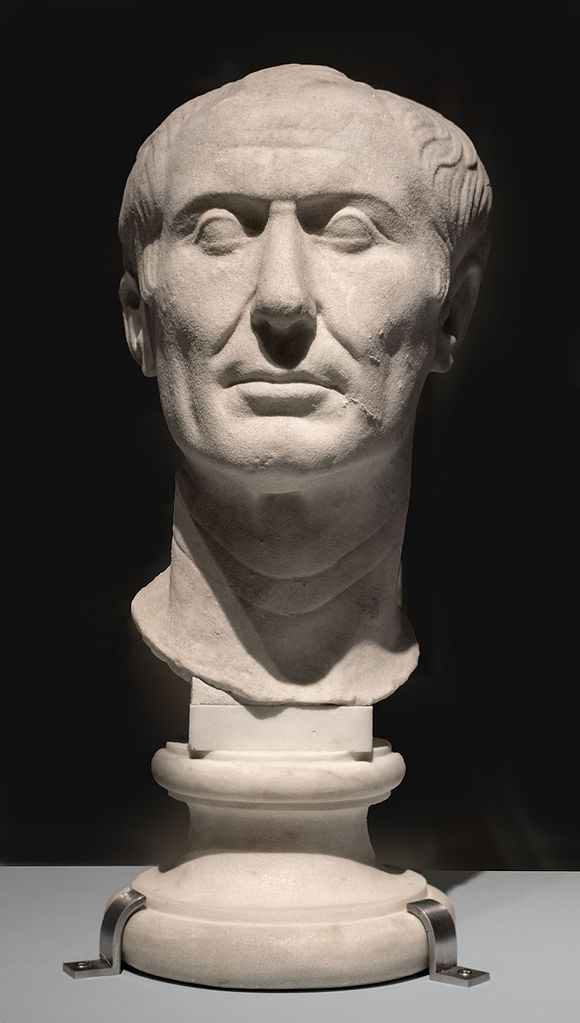
\includegraphics[width=0.5\textwidth]{figures/ceasar.jpg}\\
				\hspace*{15pt}\hbox{\scriptsize Image By:\thinspace{\itshape Ángel M. Felicísimo}}
				%https://commons.wikimedia.org/wiki/File:Retrato_de_Julio_C%C3%A9sar_(26724093101).jpg
			\end{center}

			\column{0.455\textwidth}
			\begin{center}
				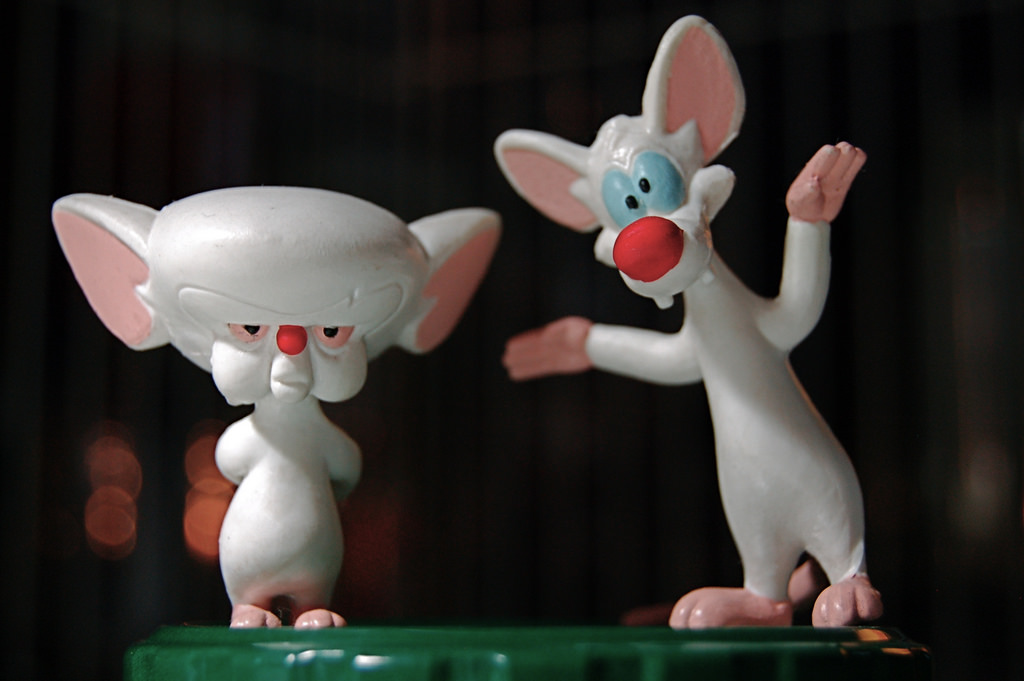
\includegraphics[width=0.9\textwidth]{figures/pinky.jpg}\\
				\hspace*{15pt}\hbox{\scriptsize Image By:\thinspace{\itshape JD Hancock}}
				%https://commons.wikimedia.org/wiki/File:Retrato_de_Julio_C%C3%A9sar_(26724093101).jpg

			\end{center}
		\end{columns}
\end{frame}

\begin{frame}
	\frametitle{Ideas for an algorithm}

	\begin{overlayarea}{\textwidth}{\textheight}
		\begin{figure}[htpb]
\begin{center}
\begin{tikzpicture}[scale=0.5, transform shape]
	\draw (-8,-3) rectangle (8,3);

	\foreach \x/\y/\name in {
		-7/2/,
		-6/1/l1,
		-5/1/l2,
		-3/-2/c1,
		-1/-2/c2,
		3/-1/,
		5/1.5/r1,
		5/0/r2,
		}{
		\node[circle, black, draw, fill=blue!30, minimum size=4pt] (\name) at (\x,\y) {};
	}
		\node at (-1.5, -3.5) {};
	\only<2->{
		\draw[dotted] (-1.5,-3) -- (-1.5,3);
		\node at (-1.5, -3.5) {\Large $L$};
	}
	\only<3->{
		\draw[dotted, red, thick] (l1) --  node[anchor=south] {\Large 1} (l2);
		\draw[dotted, red, thick] (r1) --  node[anchor=west] {\Large 1.5} (r2);
	}
	\only<4->{
		\draw[dotted, red, thick] (c1) --  node[anchor=south] {\Large 2} (c2);
	}
\end{tikzpicture}
\end{center}
\end{figure}

		
		\pause
		\begin{exampleblock}{Algorithm}
			\begin{itemize}
				\item \alert<2>{Divide}: Draw vertical line $L$ that has roughly half of the points on each side.
					\pause
				\item \alert<3>{Conquer}: Find the closest pair on each side.
					\pause
				\item \alert<4>{Combine}: Find the closest pair with one point on each side.
					\pause
				\item Return the minimum of these 3.
			\end{itemize}
		\end{exampleblock}	
	\end{overlayarea}
\end{frame}

\begin{frame}
	\frametitle{Did we make things better?}
	\begin{questionblock}{What is the run time of combine?}
		How much time to combine the two halves? Remember that we want to improve over $\Theta(n^2)$.
	\end{questionblock}	
\end{frame}

\begin{frame}
	\frametitle{How do we make it better?}
		\begin{figure}[htpb]
\begin{center}
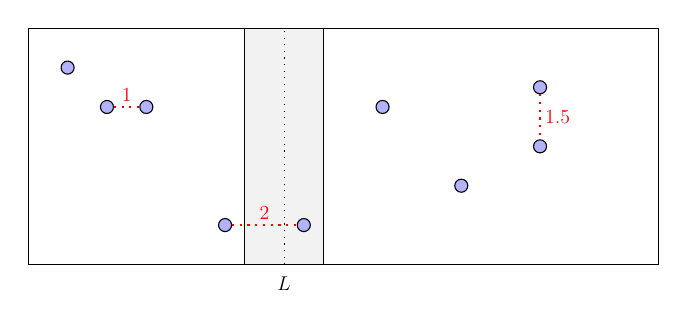
\begin{tikzpicture}[scale=0.5, transform shape]
	\draw (-8,-3) rectangle (8,3);

	\only<2->{
		\draw[fill=gray!10] (-2.5,-3) rectangle (-0.5,3);
	}
	\foreach \x/\y/\name in {
		-7/2/,
		-6/1/l1,
		-5/1/l2,
		-3/-2/c1,
		-1/-2/c2,
		3/-1/,
		5/1.5/r1,
		5/0/r2,
		}{
		\node[circle, black, draw, fill=blue!30, minimum size=4pt] (\name) at (\x,\y) {};
	}
		\draw[dotted] (-1.5,-3) -- (-1.5,3);
		\node at (-1.5, -3.5) {\Large $L$};
		\draw[dotted, red, thick] (l1) --  node[anchor=south] {\Large 1} (l2);
		\draw[dotted, red, thick] (r1) --  node[anchor=west] {\Large 1.5} (r2);
		\draw[dotted, red, thick] (c1) --  node[anchor=south] {\Large 2} (c2);

\end{tikzpicture}
\end{center}
\end{figure}

	Observation:
	\begin{itemize}
		\item If $\delta$ is the minimum of the smallest distances left and right.
			\pause
		\item Then we only need to consider pairs of points within $\delta$ of $L$.
			\pause
		\item So in this example, none at all!
	\end{itemize}
\end{frame}

\begin{frame}
	\frametitle{Worst-case?}
	\begin{overlayarea}{\textwidth}{\textheight}
			\begin{itemize}
				\item But worst-case all points are in this $2\delta$-strip...
					\pause
				\item But if we sort them by $y$-coordinate (which can be done in $O(n\log n)$), then how many comparisons do we need?
					\pause
				\item Still $O(n^2)$!?
					\only<4->{
				\item Nope! We only need to check within 11 (i.e. a constant number of) positions in the sorted list.
				}
					\only<5->{
				\item So the combining step is $O(n \log n)$ (which can be further improved to $O(n)$)!
				}
			\end{itemize}
			\only<3>{
			\begin{center}
				
\includegraphics[width=0.4\textwidth]{figures/dilbert.jpg}
				\framesubtitle{http://thecontextofthings.com/wp-content/uploads/2017/11/dilbert-work.jpg}
			\end{center}
		}
	\end{overlayarea}
\end{frame}

\begin{frame}
	\frametitle{Why 11?}

	\begin{overlayarea}{\textwidth}{\textheight}
		\begin{columns}
			\column{0.655\textwidth}
			\begin{block}{Definition}
				Let $s_i$ be the point in the $2\delta$-strip with the $i^\text{th}$ smallest $y$-coordinate.
			\end{block}	
			
			\pause
			\begin{block}{Claim about 11}
				If $|i-j| > 11$ then the distance between $s_i$ and $s_j$ is at least $\delta$.
			\end{block}
			\column{0.255\textwidth}
			\begin{figure}[htpb]
\begin{center}
\begin{tikzpicture}[scale=0.4, transform shape]
	\draw (-2,-4) rectangle (2,4);
	
	\only<5->{
		\foreach \y in {-2, ..., 0}{
			\foreach \x in {-2, ..., 1}{
				\draw[fill=green!30] (\x,\y) rectangle (\x+1,\y+1);
			}
		}
	}

	\foreach \x/\y/\name/\color in {
		1.35/-2.4/1/red,
		-1.35/-1.6/2/green,
		-0.4/-0.4/3/blue,
		1.3/0.5/4/blue,
	%	1.7/1.4/5/red,
		-0.4/2.4/5/red,
		0.3/2.4/6/red}{
		\alt<4->{
		\node[circle, black, draw, fill=\color!30, minimum size=4pt] () at (\x,\y) {\name};
			}{
		\node[circle, black, draw, fill=blue!30, minimum size=4pt] () at (\x,\y) {\name};
		}
	}
		\draw[thick] (0,-4) -- (0,4);
		\node at (0, -4.5) {\Large $L$};
		\node at (-2, -4.5) {\Large $L-\delta$};
		\node at (2, -4.5) {\Large $L+\delta$};
		\only<3->{
			\draw[dotted] (1,-4) -- (1,4);
			\draw[dotted] (-1,-4) -- (-1,4);

			\foreach \y in {-3, ..., 3}{
				\draw[dotted] (-2,\y) -- (2,\y);
			}
		}

\end{tikzpicture}
\end{center}
\end{figure}
	
		\end{columns}
		
		\pause
		\only<3-5>{
			\begin{block}{Proof sketch}
			\begin{itemize}
				\item No two points are in the same $0.5\delta$-by-$0.5\delta$-box.
					\only<4->{
				\item Two points that have two rows between them have a distance $\geq 2\cdot(0.5\delta) = \delta$.
				}
				\only<5->{
				\item So we only consider points at most 2 rows away.
				}
			\end{itemize}
		\end{block}
	}
	\only<6->{
		\begin{exampleblock}{Fun facts!}
			\begin{itemize}
				\item We can even reduce this to just 7 points.
					\only<7>{
				\item Even less if we consider columns separately.
				}
			\end{itemize}
		\end{exampleblock}	
	}
		
		\only<3>{
		\begin{questionblock}{Why not?}
			Why are there no two points in the same box?
		\end{questionblock}
}
	\end{overlayarea}
\end{frame}

\begin{frame}
	\frametitle{The algorithm}
	\begin{columns}
		\column{0.705\textwidth}
	\begin{algorithmic}
		\State Sort all points by x-coordinate
		\Function{Closest-Pair}{$p_1,\dots,p_n$}
			\If{n=1}
				\State \Return $\infty$
			\EndIf

			\pause
			\State $L \gets$ \alert<2>{median} $x$-coordinate
			\State $\delta_1 \gets$ \Call{Closest-Pair}{Points left of $L$}
			\State $\delta_2 \gets$ \Call{Closest-Pair}{Points right of $L$}
			\State $\delta \gets \min(\delta_1,\delta_2)$
			\pause
			\State get list of all points within $\delta$ from L.
			\State sort this list by y-coordinate
			\pause
			\State Scan by y-order, compare every point to the next 11 and update $\delta$ as you go.
			\State \Return $\delta$
		\EndFunction
	\end{algorithmic}
		\pnote{Why not the average?}
		\column{0.205\textwidth}
		\pause
		\begin{questionblock}{}
			What is the recurrence equation for the run time?	
		\end{questionblock}	
		\pause
		\begin{answerblock}{}
			\small
			$T(n) =2T(n/2) + O(n\log n)$	
		\end{answerblock}
	\end{columns}
	
\end{frame}

		\begin{questionblock}{Brute-force}
			What is the tightest upper bound on the run time for a brute-force solution given $|S| = n$?
			\only<2>{
			\begin{enumerate}[A.]
				\item $O(n \log n)$
				\item $O(n^2)$
				\item $O(n^2 \log n)$
				\item $O(n^3)$
				\item I don't know.
			\end{enumerate}
		}
		\end{questionblock}
		\only<3>{
			\begin{answerblock}{Try every combination}
				We check every pair of points, of which there are $n^2$, so $O(n^2)$.	
			\end{answerblock}
		}
	\end{overlayarea}
\end{frame}

\begin{frame}
	\frametitle{Time to improve!}
	\framesubtitle{Using Divide \& Conquer}
		\begin{columns}
			\column{0.455\textwidth}
			\begin{center}
				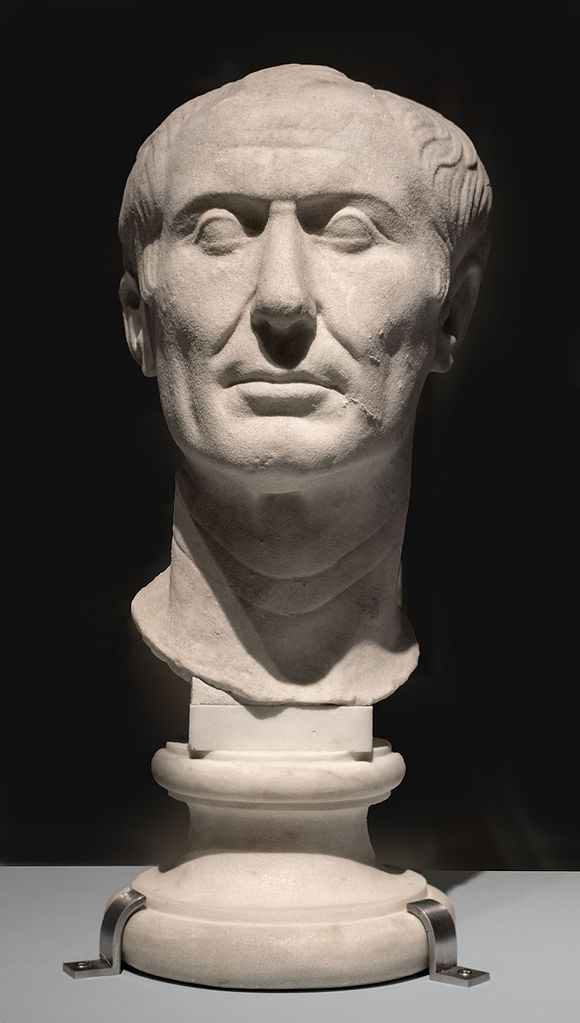
\includegraphics[width=0.5\textwidth]{figures/ceasar.jpg}\\
				\hspace*{15pt}\hbox{\scriptsize Image By:\thinspace{\itshape Ángel M. Felicísimo}}
				%https://commons.wikimedia.org/wiki/File:Retrato_de_Julio_C%C3%A9sar_(26724093101).jpg
			\end{center}

			\column{0.455\textwidth}
			\begin{center}
				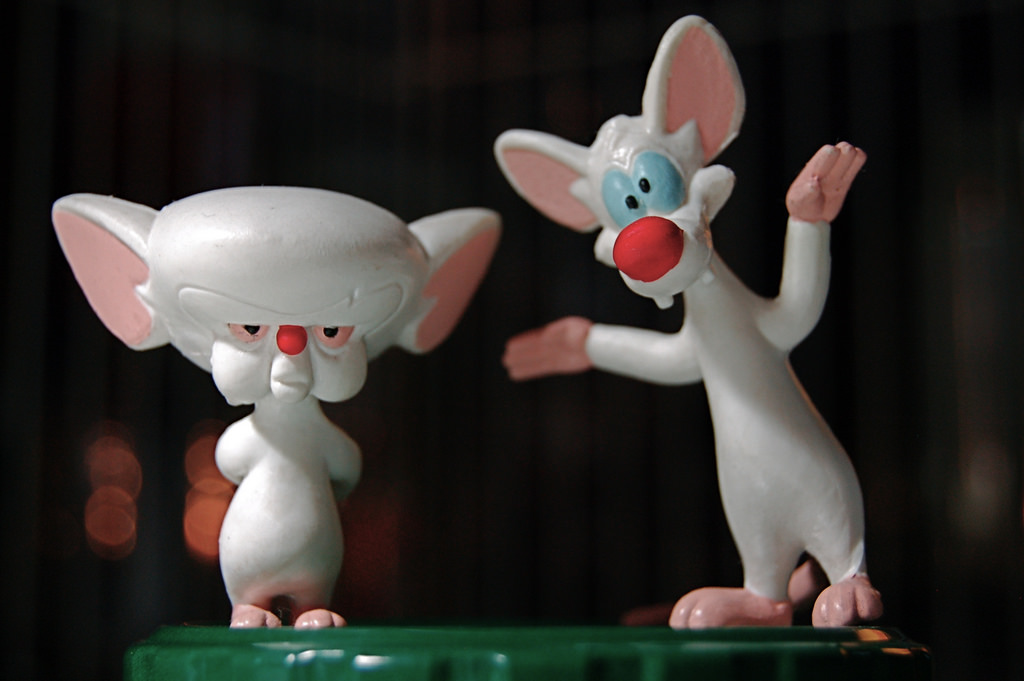
\includegraphics[width=0.9\textwidth]{figures/pinky.jpg}\\
				\hspace*{15pt}\hbox{\scriptsize Image By:\thinspace{\itshape JD Hancock}}
				%https://commons.wikimedia.org/wiki/File:Retrato_de_Julio_C%C3%A9sar_(26724093101).jpg

			\end{center}
		\end{columns}
\end{frame}

\begin{frame}
	\frametitle{Ideas for an algorithm}

	\begin{overlayarea}{\textwidth}{\textheight}
		\begin{figure}[htpb]
\begin{center}
\begin{tikzpicture}[scale=0.5, transform shape]
	\draw (-8,-3) rectangle (8,3);

	\foreach \x/\y/\name in {
		-7/2/,
		-6/1/l1,
		-5/1/l2,
		-3/-2/c1,
		-1/-2/c2,
		3/-1/,
		5/1.5/r1,
		5/0/r2,
		}{
		\node[circle, black, draw, fill=blue!30, minimum size=4pt] (\name) at (\x,\y) {};
	}
		\node at (-1.5, -3.5) {};
	\only<2->{
		\draw[dotted] (-1.5,-3) -- (-1.5,3);
		\node at (-1.5, -3.5) {\Large $L$};
	}
	\only<3->{
		\draw[dotted, red, thick] (l1) --  node[anchor=south] {\Large 1} (l2);
		\draw[dotted, red, thick] (r1) --  node[anchor=west] {\Large 1.5} (r2);
	}
	\only<4->{
		\draw[dotted, red, thick] (c1) --  node[anchor=south] {\Large 2} (c2);
	}
\end{tikzpicture}
\end{center}
\end{figure}

		
		\pause
		\begin{exampleblock}{Algorithm}
			\begin{itemize}
				\item \alert<2>{Divide}: Draw vertical line $L$ that has roughly half of the points on each side.
					\pause
				\item \alert<3>{Conquer}: Find the closest pair on each side.
					\pause
				\item \alert<4>{Combine}: Find the closest pair with one point on each side.
					\pause
				\item Return the minimum of these 3.
			\end{itemize}
		\end{exampleblock}	
	\end{overlayarea}
\end{frame}

\begin{frame}
	\frametitle{Did we make things better?}
	\begin{questionblock}{What is the run time of combine?}
		How much time to combine the two halves? Remember that we want to improve over $\Theta(n^2)$.
	\end{questionblock}	
\end{frame}

\begin{frame}
	\frametitle{How do we make it better?}
		\begin{figure}[htpb]
\begin{center}
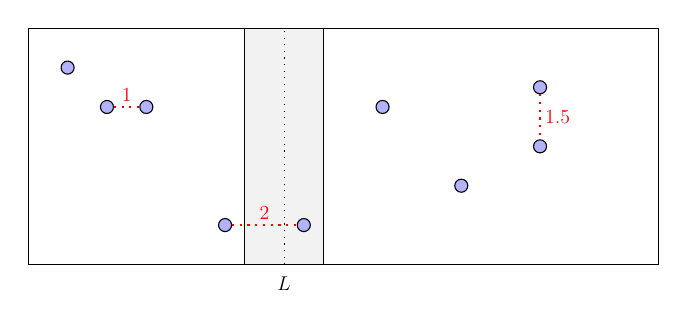
\begin{tikzpicture}[scale=0.5, transform shape]
	\draw (-8,-3) rectangle (8,3);

	\only<2->{
		\draw[fill=gray!10] (-2.5,-3) rectangle (-0.5,3);
	}
	\foreach \x/\y/\name in {
		-7/2/,
		-6/1/l1,
		-5/1/l2,
		-3/-2/c1,
		-1/-2/c2,
		3/-1/,
		5/1.5/r1,
		5/0/r2,
		}{
		\node[circle, black, draw, fill=blue!30, minimum size=4pt] (\name) at (\x,\y) {};
	}
		\draw[dotted] (-1.5,-3) -- (-1.5,3);
		\node at (-1.5, -3.5) {\Large $L$};
		\draw[dotted, red, thick] (l1) --  node[anchor=south] {\Large 1} (l2);
		\draw[dotted, red, thick] (r1) --  node[anchor=west] {\Large 1.5} (r2);
		\draw[dotted, red, thick] (c1) --  node[anchor=south] {\Large 2} (c2);

\end{tikzpicture}
\end{center}
\end{figure}

	Observation:
	\begin{itemize}
		\item If $\delta$ is the minimum of the smallest distances left and right.
			\pause
		\item Then we only need to consider pairs of points within $\delta$ of $L$.
			\pause
		\item So in this example, none at all!
	\end{itemize}
\end{frame}

\begin{frame}
	\frametitle{Worst-case?}
	\begin{overlayarea}{\textwidth}{\textheight}
			\begin{itemize}
				\item But worst-case all points are in this $2\delta$-strip...
					\pause
				\item But if we sort them by $y$-coordinate (which can be done in $O(n\log n)$), then how many comparisons do we need?
					\pause
				\item Still $O(n^2)$!?
					\only<4->{
				\item Nope! We only need to check within 11 (i.e. a constant number of) positions in the sorted list.
				}
					\only<5->{
				\item So the combining step is $O(n \log n)$ (which can be further improved to $O(n)$)!
				}
			\end{itemize}
			\only<3>{
			\begin{center}
				
\includegraphics[width=0.4\textwidth]{figures/dilbert.jpg}
				\framesubtitle{http://thecontextofthings.com/wp-content/uploads/2017/11/dilbert-work.jpg}
			\end{center}
		}
	\end{overlayarea}
\end{frame}

\begin{frame}
	\frametitle{Why 11?}

	\begin{overlayarea}{\textwidth}{\textheight}
		\begin{columns}
			\column{0.655\textwidth}
			\begin{block}{Definition}
				Let $s_i$ be the point in the $2\delta$-strip with the $i^\text{th}$ smallest $y$-coordinate.
			\end{block}	
			
			\pause
			\begin{block}{Claim about 11}
				If $|i-j| > 11$ then the distance between $s_i$ and $s_j$ is at least $\delta$.
			\end{block}
			\column{0.255\textwidth}
			\begin{figure}[htpb]
\begin{center}
\begin{tikzpicture}[scale=0.4, transform shape]
	\draw (-2,-4) rectangle (2,4);
	
	\only<5->{
		\foreach \y in {-2, ..., 0}{
			\foreach \x in {-2, ..., 1}{
				\draw[fill=green!30] (\x,\y) rectangle (\x+1,\y+1);
			}
		}
	}

	\foreach \x/\y/\name/\color in {
		1.35/-2.4/1/red,
		-1.35/-1.6/2/green,
		-0.4/-0.4/3/blue,
		1.3/0.5/4/blue,
	%	1.7/1.4/5/red,
		-0.4/2.4/5/red,
		0.3/2.4/6/red}{
		\alt<4->{
		\node[circle, black, draw, fill=\color!30, minimum size=4pt] () at (\x,\y) {\name};
			}{
		\node[circle, black, draw, fill=blue!30, minimum size=4pt] () at (\x,\y) {\name};
		}
	}
		\draw[thick] (0,-4) -- (0,4);
		\node at (0, -4.5) {\Large $L$};
		\node at (-2, -4.5) {\Large $L-\delta$};
		\node at (2, -4.5) {\Large $L+\delta$};
		\only<3->{
			\draw[dotted] (1,-4) -- (1,4);
			\draw[dotted] (-1,-4) -- (-1,4);

			\foreach \y in {-3, ..., 3}{
				\draw[dotted] (-2,\y) -- (2,\y);
			}
		}

\end{tikzpicture}
\end{center}
\end{figure}
	
		\end{columns}
		
		\pause
		\only<3-5>{
			\begin{block}{Proof sketch}
			\begin{itemize}
				\item No two points are in the same $0.5\delta$-by-$0.5\delta$-box.
					\only<4->{
				\item Two points that have two rows between them have a distance $\geq 2\cdot(0.5\delta) = \delta$.
				}
				\only<5->{
				\item So we only consider points at most 2 rows away.
				}
			\end{itemize}
		\end{block}
	}
	\only<6->{
		\begin{exampleblock}{Fun facts!}
			\begin{itemize}
				\item We can even reduce this to just 7 points.
					\only<7>{
				\item Even less if we consider columns separately.
				}
			\end{itemize}
		\end{exampleblock}	
	}
		
		\only<3>{
		\begin{questionblock}{Why not?}
			Why are there no two points in the same box?
		\end{questionblock}
}
	\end{overlayarea}
\end{frame}

\begin{frame}
	\frametitle{The algorithm}
	\begin{columns}
		\column{0.705\textwidth}
	\begin{algorithmic}
		\State Sort all points by x-coordinate
		\Function{Closest-Pair}{$p_1,\dots,p_n$}
			\If{n=1}
				\State \Return $\infty$
			\EndIf

			\pause
			\State $L \gets$ \alert<2>{median} $x$-coordinate
			\State $\delta_1 \gets$ \Call{Closest-Pair}{Points left of $L$}
			\State $\delta_2 \gets$ \Call{Closest-Pair}{Points right of $L$}
			\State $\delta \gets \min(\delta_1,\delta_2)$
			\pause
			\State get list of all points within $\delta$ from L.
			\State sort this list by y-coordinate
			\pause
			\State Scan by y-order, compare every point to the next 11 and update $\delta$ as you go.
			\State \Return $\delta$
		\EndFunction
	\end{algorithmic}
		\pnote{Why not the average?}
		\column{0.205\textwidth}
		\pause
		\begin{questionblock}{}
			What is the recurrence equation for the run time?	
		\end{questionblock}	
		\pause
		\begin{answerblock}{}
			\small
			$T(n) =2T(n/2) + O(n\log n)$	
		\end{answerblock}
	\end{columns}
	
\end{frame}

		\begin{questionblock}{Brute-force}
			What is the tightest upper bound on the run time for a brute-force solution given $|S| = n$?
			\only<2>{
			\begin{enumerate}[A.]
				\item $O(n \log n)$
				\item $O(n^2)$
				\item $O(n^2 \log n)$
				\item $O(n^3)$
				\item I don't know.
			\end{enumerate}
		}
		\end{questionblock}
		\only<3>{
			\begin{answerblock}{Try every combination}
				We check every pair of points, of which there are $n^2$, so $O(n^2)$.	
			\end{answerblock}
		}
	\end{overlayarea}
\end{frame}

\begin{frame}
	\frametitle{Time to improve!}
	\framesubtitle{Using Divide \& Conquer}
		\begin{columns}
			\column{0.455\textwidth}
			\begin{center}
				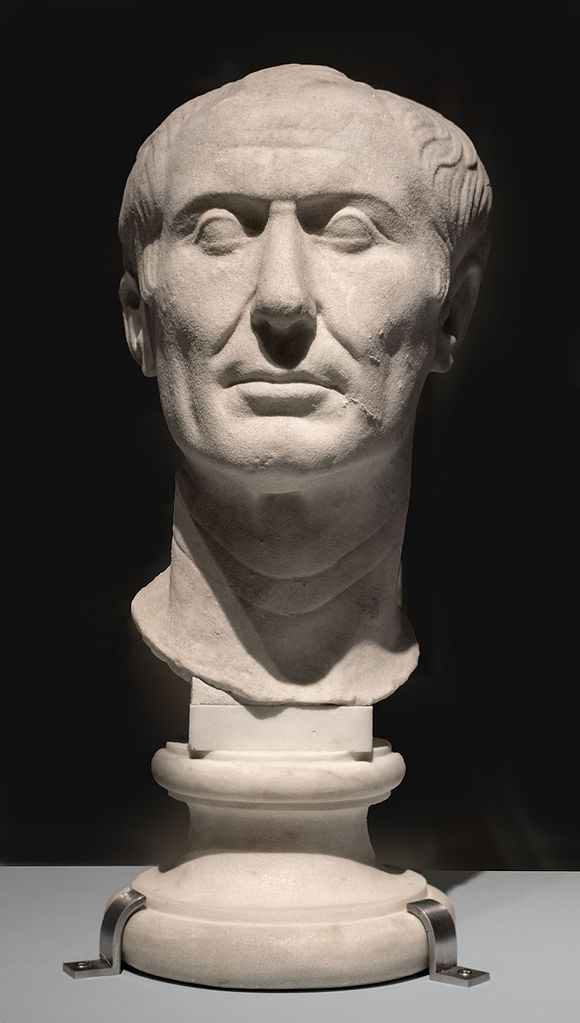
\includegraphics[width=0.5\textwidth]{figures/ceasar.jpg}\\
				\hspace*{15pt}\hbox{\scriptsize Image By:\thinspace{\itshape Ángel M. Felicísimo}}
				%https://commons.wikimedia.org/wiki/File:Retrato_de_Julio_C%C3%A9sar_(26724093101).jpg
			\end{center}

			\column{0.455\textwidth}
			\begin{center}
				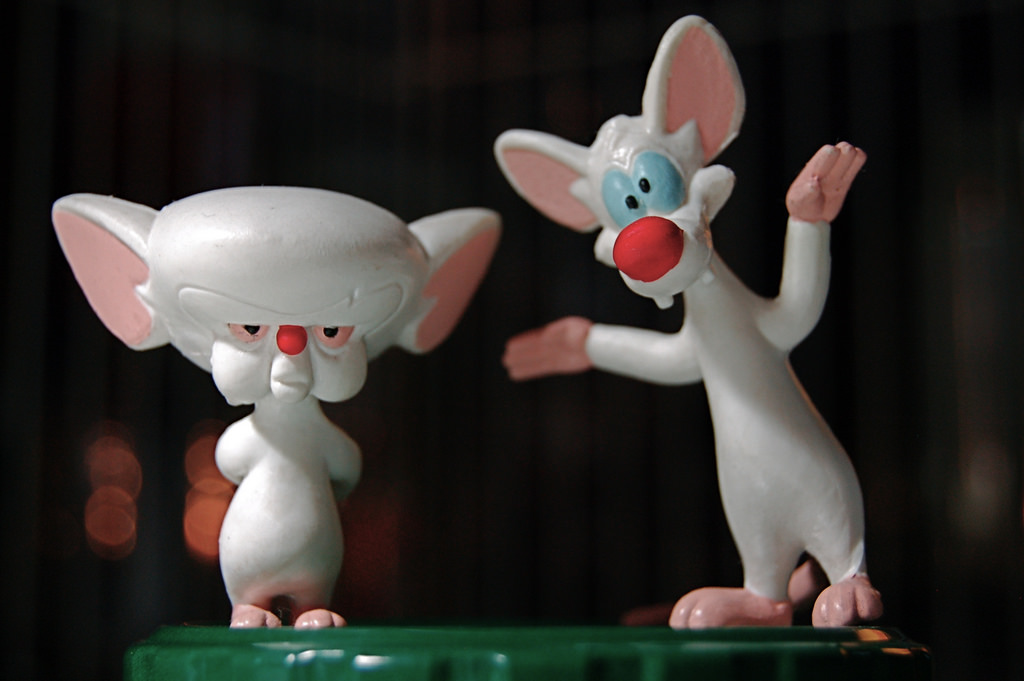
\includegraphics[width=0.9\textwidth]{figures/pinky.jpg}\\
				\hspace*{15pt}\hbox{\scriptsize Image By:\thinspace{\itshape JD Hancock}}
				%https://commons.wikimedia.org/wiki/File:Retrato_de_Julio_C%C3%A9sar_(26724093101).jpg

			\end{center}
		\end{columns}
\end{frame}

\begin{frame}
	\frametitle{Ideas for an algorithm}

	\begin{overlayarea}{\textwidth}{\textheight}
		\begin{figure}[htpb]
\begin{center}
\begin{tikzpicture}[scale=0.5, transform shape]
	\draw (-8,-3) rectangle (8,3);

	\foreach \x/\y/\name in {
		-7/2/,
		-6/1/l1,
		-5/1/l2,
		-3/-2/c1,
		-1/-2/c2,
		3/-1/,
		5/1.5/r1,
		5/0/r2,
		}{
		\node[circle, black, draw, fill=blue!30, minimum size=4pt] (\name) at (\x,\y) {};
	}
		\node at (-1.5, -3.5) {};
	\only<2->{
		\draw[dotted] (-1.5,-3) -- (-1.5,3);
		\node at (-1.5, -3.5) {\Large $L$};
	}
	\only<3->{
		\draw[dotted, red, thick] (l1) --  node[anchor=south] {\Large 1} (l2);
		\draw[dotted, red, thick] (r1) --  node[anchor=west] {\Large 1.5} (r2);
	}
	\only<4->{
		\draw[dotted, red, thick] (c1) --  node[anchor=south] {\Large 2} (c2);
	}
\end{tikzpicture}
\end{center}
\end{figure}

		
		\pause
		\begin{exampleblock}{Algorithm}
			\begin{itemize}
				\item \alert<2>{Divide}: Draw vertical line $L$ that has roughly half of the points on each side.
					\pause
				\item \alert<3>{Conquer}: Find the closest pair on each side.
					\pause
				\item \alert<4>{Combine}: Find the closest pair with one point on each side.
					\pause
				\item Return the minimum of these 3.
			\end{itemize}
		\end{exampleblock}	
	\end{overlayarea}
\end{frame}

\begin{frame}
	\frametitle{Did we make things better?}
	\begin{questionblock}{What is the run time of combine?}
		How much time to combine the two halves? Remember that we want to improve over $\Theta(n^2)$.
	\end{questionblock}	
\end{frame}

\begin{frame}
	\frametitle{How do we make it better?}
		\begin{figure}[htpb]
\begin{center}
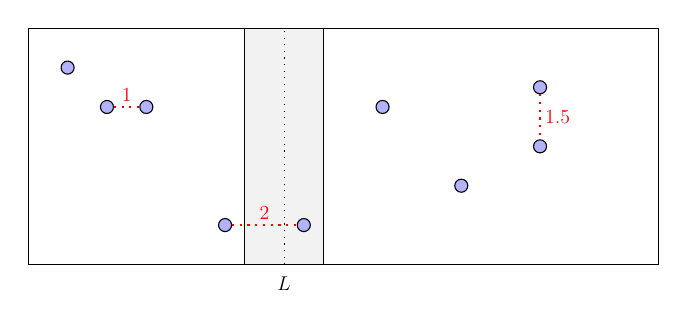
\begin{tikzpicture}[scale=0.5, transform shape]
	\draw (-8,-3) rectangle (8,3);

	\only<2->{
		\draw[fill=gray!10] (-2.5,-3) rectangle (-0.5,3);
	}
	\foreach \x/\y/\name in {
		-7/2/,
		-6/1/l1,
		-5/1/l2,
		-3/-2/c1,
		-1/-2/c2,
		3/-1/,
		5/1.5/r1,
		5/0/r2,
		}{
		\node[circle, black, draw, fill=blue!30, minimum size=4pt] (\name) at (\x,\y) {};
	}
		\draw[dotted] (-1.5,-3) -- (-1.5,3);
		\node at (-1.5, -3.5) {\Large $L$};
		\draw[dotted, red, thick] (l1) --  node[anchor=south] {\Large 1} (l2);
		\draw[dotted, red, thick] (r1) --  node[anchor=west] {\Large 1.5} (r2);
		\draw[dotted, red, thick] (c1) --  node[anchor=south] {\Large 2} (c2);

\end{tikzpicture}
\end{center}
\end{figure}

	Observation:
	\begin{itemize}
		\item If $\delta$ is the minimum of the smallest distances left and right.
			\pause
		\item Then we only need to consider pairs of points within $\delta$ of $L$.
			\pause
		\item So in this example, none at all!
	\end{itemize}
\end{frame}

\begin{frame}
	\frametitle{Worst-case?}
	\begin{overlayarea}{\textwidth}{\textheight}
			\begin{itemize}
				\item But worst-case all points are in this $2\delta$-strip...
					\pause
				\item But if we sort them by $y$-coordinate (which can be done in $O(n\log n)$), then how many comparisons do we need?
					\pause
				\item Still $O(n^2)$!?
					\only<4->{
				\item Nope! We only need to check within 11 (i.e. a constant number of) positions in the sorted list.
				}
					\only<5->{
				\item So the combining step is $O(n \log n)$ (which can be further improved to $O(n)$)!
				}
			\end{itemize}
			\only<3>{
			\begin{center}
				
\includegraphics[width=0.4\textwidth]{figures/dilbert.jpg}
				\framesubtitle{http://thecontextofthings.com/wp-content/uploads/2017/11/dilbert-work.jpg}
			\end{center}
		}
	\end{overlayarea}
\end{frame}

\begin{frame}
	\frametitle{Why 11?}

	\begin{overlayarea}{\textwidth}{\textheight}
		\begin{columns}
			\column{0.655\textwidth}
			\begin{block}{Definition}
				Let $s_i$ be the point in the $2\delta$-strip with the $i^\text{th}$ smallest $y$-coordinate.
			\end{block}	
			
			\pause
			\begin{block}{Claim about 11}
				If $|i-j| > 11$ then the distance between $s_i$ and $s_j$ is at least $\delta$.
			\end{block}
			\column{0.255\textwidth}
			\begin{figure}[htpb]
\begin{center}
\begin{tikzpicture}[scale=0.4, transform shape]
	\draw (-2,-4) rectangle (2,4);
	
	\only<5->{
		\foreach \y in {-2, ..., 0}{
			\foreach \x in {-2, ..., 1}{
				\draw[fill=green!30] (\x,\y) rectangle (\x+1,\y+1);
			}
		}
	}

	\foreach \x/\y/\name/\color in {
		1.35/-2.4/1/red,
		-1.35/-1.6/2/green,
		-0.4/-0.4/3/blue,
		1.3/0.5/4/blue,
	%	1.7/1.4/5/red,
		-0.4/2.4/5/red,
		0.3/2.4/6/red}{
		\alt<4->{
		\node[circle, black, draw, fill=\color!30, minimum size=4pt] () at (\x,\y) {\name};
			}{
		\node[circle, black, draw, fill=blue!30, minimum size=4pt] () at (\x,\y) {\name};
		}
	}
		\draw[thick] (0,-4) -- (0,4);
		\node at (0, -4.5) {\Large $L$};
		\node at (-2, -4.5) {\Large $L-\delta$};
		\node at (2, -4.5) {\Large $L+\delta$};
		\only<3->{
			\draw[dotted] (1,-4) -- (1,4);
			\draw[dotted] (-1,-4) -- (-1,4);

			\foreach \y in {-3, ..., 3}{
				\draw[dotted] (-2,\y) -- (2,\y);
			}
		}

\end{tikzpicture}
\end{center}
\end{figure}
	
		\end{columns}
		
		\pause
		\only<3-5>{
			\begin{block}{Proof sketch}
			\begin{itemize}
				\item No two points are in the same $0.5\delta$-by-$0.5\delta$-box.
					\only<4->{
				\item Two points that have two rows between them have a distance $\geq 2\cdot(0.5\delta) = \delta$.
				}
				\only<5->{
				\item So we only consider points at most 2 rows away.
				}
			\end{itemize}
		\end{block}
	}
	\only<6->{
		\begin{exampleblock}{Fun facts!}
			\begin{itemize}
				\item We can even reduce this to just 7 points.
					\only<7>{
				\item Even less if we consider columns separately.
				}
			\end{itemize}
		\end{exampleblock}	
	}
		
		\only<3>{
		\begin{questionblock}{Why not?}
			Why are there no two points in the same box?
		\end{questionblock}
}
	\end{overlayarea}
\end{frame}

\begin{frame}
	\frametitle{The algorithm}
	\begin{columns}
		\column{0.705\textwidth}
	\begin{algorithmic}
		\State Sort all points by x-coordinate
		\Function{Closest-Pair}{$p_1,\dots,p_n$}
			\If{n=1}
				\State \Return $\infty$
			\EndIf

			\pause
			\State $L \gets$ \alert<2>{median} $x$-coordinate
			\State $\delta_1 \gets$ \Call{Closest-Pair}{Points left of $L$}
			\State $\delta_2 \gets$ \Call{Closest-Pair}{Points right of $L$}
			\State $\delta \gets \min(\delta_1,\delta_2)$
			\pause
			\State get list of all points within $\delta$ from L.
			\State sort this list by y-coordinate
			\pause
			\State Scan by y-order, compare every point to the next 11 and update $\delta$ as you go.
			\State \Return $\delta$
		\EndFunction
	\end{algorithmic}
		\pnote{Why not the average?}
		\column{0.205\textwidth}
		\pause
		\begin{questionblock}{}
			What is the recurrence equation for the run time?	
		\end{questionblock}	
		\pause
		\begin{answerblock}{}
			\small
			$T(n) =2T(n/2) + O(n\log n)$	
		\end{answerblock}
	\end{columns}
	
\end{frame}
